\chapter{Physical Layer}
\chapterminitoc

\section{Fundamentals of Data Signals}

\subsection{Physical Representation of Data}

\noindent
Signal $\rightarrow$ a physical representation of data.

\begin{itemize}
    \item Analog signal (continuous signal) $\rightarrow$ tín hiệu liên tục (continuous); biến đổi liên tục theo thời gian (ví dụ, nó sẽ chạy từ 0 đến 1, chấp nhận các giá trị trong khoảng này như 0.1, 0.01, 0.001, ...).
    \item Digital signal (discrete signal) $\rightarrow$ tín hiệu rời rạc (discrete); biến đổi theo từng bước (ví dụ, nó chỉ chấp nhận các giá trị 0 và 1).
\end{itemize}
\medskip

\begin{figure}[ht]
    \centering
    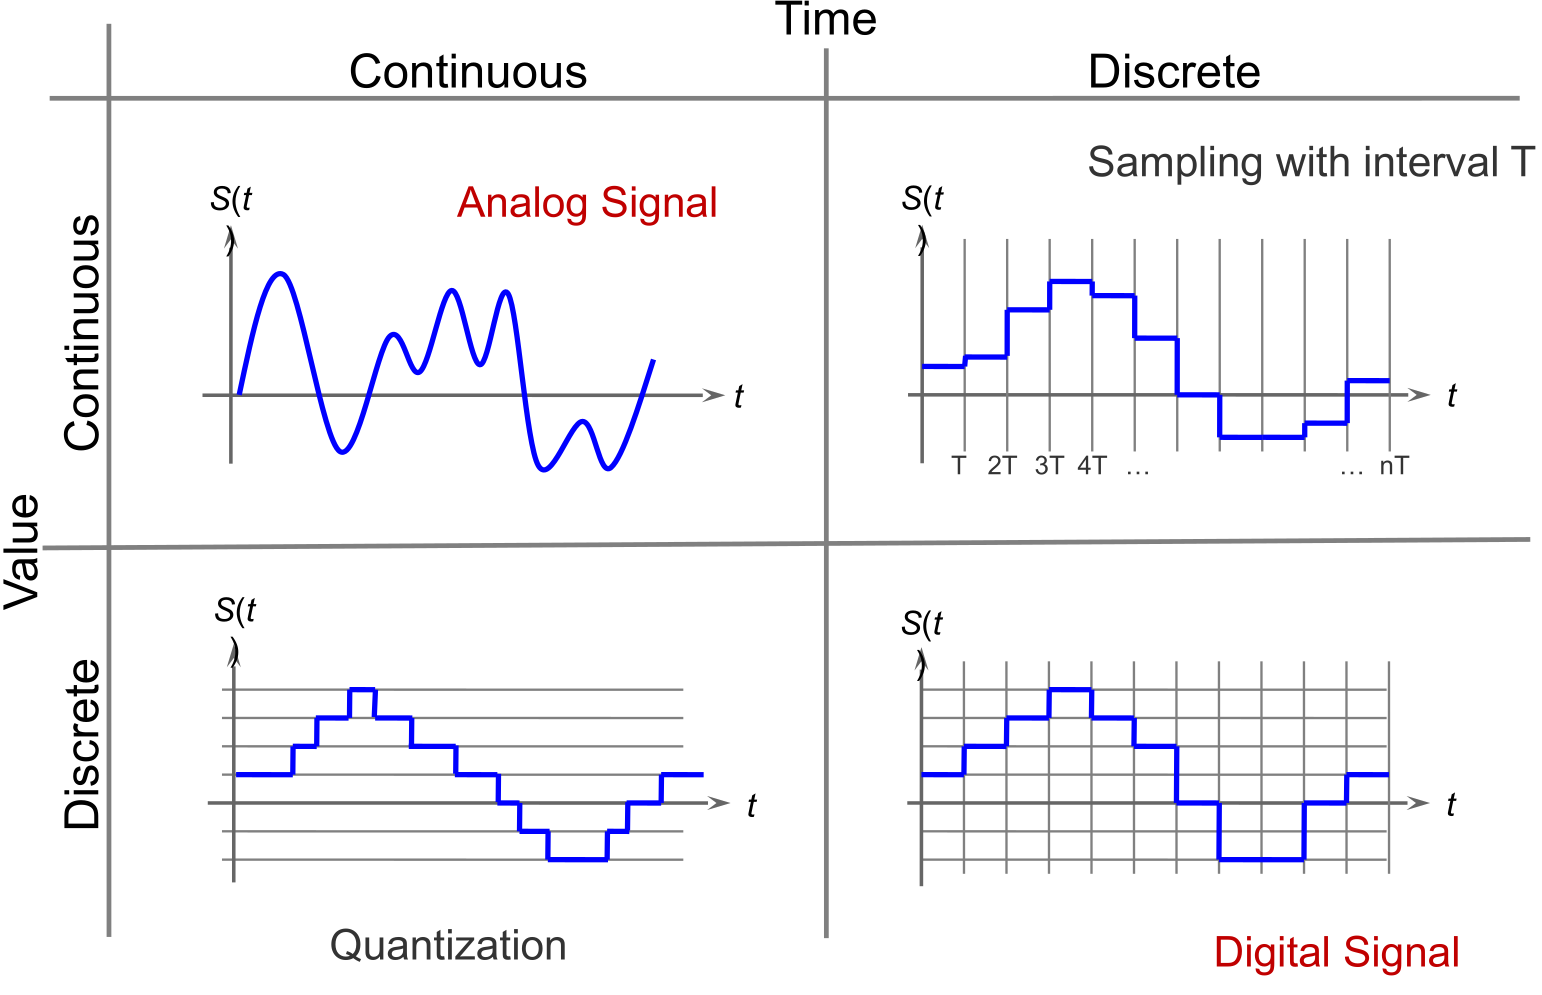
\includegraphics[width=0.8\textwidth]{assets/chap_2/cont_dis.png}
\end{figure}
\medskip

\noindent
The translator $\Rightarrow$ NIC (Network Interface Card, nghĩa là card mạng) hoạt động như bộ mã hóa và giải mã (\textbf{co}der and \textbf{dec}oder $\rightarrow$ CODEC).
\medskip

\subsection{The Telephone Example}

\begin{figure}[H]
    \centering
    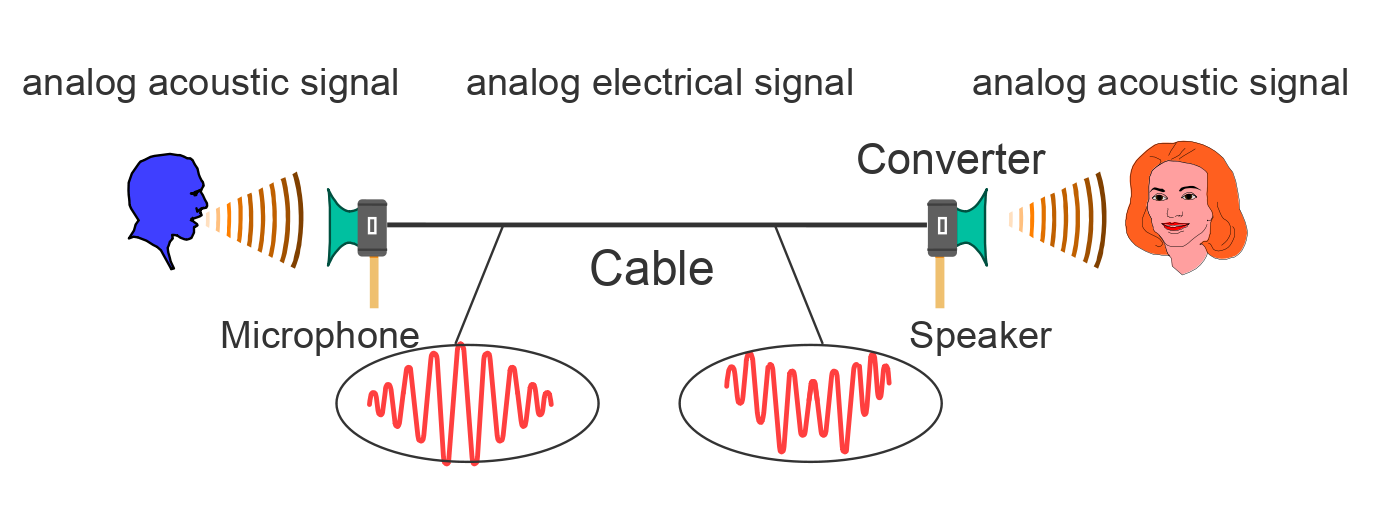
\includegraphics[width=0.7\textwidth]{assets/chap_2/telephone_ex.png}
\end{figure}
\medskip

\noindent
\underline{Giải thích:}

\begin{enumerate}
    \item Giọng nói tạo ra sóng âm (ra tín hiệu âm thanh (analog acoustic signal)) $\rightarrow$ đi qua microphone, hoạt động như như bộ chuyển đổi ($\rightarrow$ biến sóng âm thành dòng điện).
    \item Tín hiệu điện (analog electrical signal) truyền trong dây dẫn (cable) tới converter (là speaker).
    \item Ở đây, speaker sẽ biến dòng điện trở lại thành âm thanh (acoustic signal) để người nghe có thể nghe được.
\end{enumerate}

\subsection{Basics of Signal Processing}

\noindent
Periodic signal (tín hiệu tuần hoàn) $\rightarrow$ simplest signals.
\medskip

\begin{figure}[ht]
    \centering
    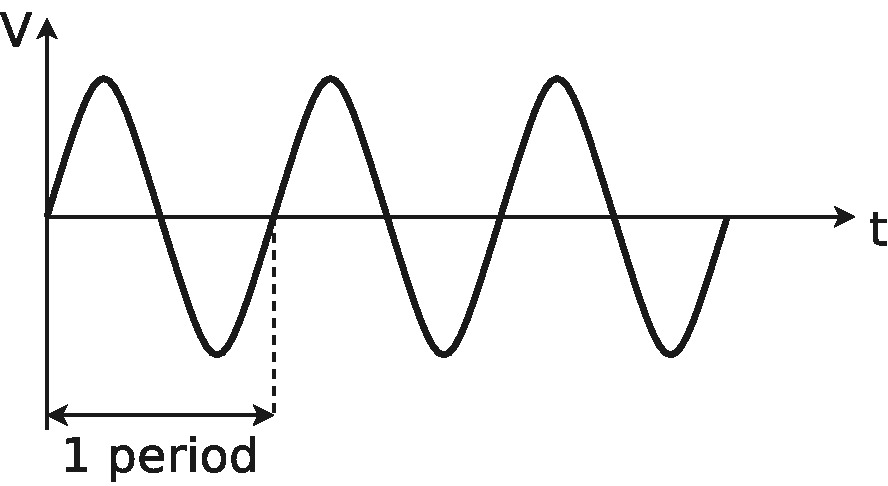
\includegraphics[width=0.4\textwidth]{assets/chap_2/wave.jpg}
\end{figure}
\medskip

\noindent
\underline{Parameters:}

\begin{itemize}
    \item Period ($T$)
    \item Frequency ($f$) $\rightarrow$ số chu kỳ trong 1 giây (Hz) $\Rightarrow$ $f = \frac{1}{T}$.
    \item Amplitude ($S(t)$) $\rightarrow$ độ lớn tín hiệu.
    \item Phase ($\phi$) $\rightarrow$ vị trí bắt đầu của sóng trong chu kỳ.
\end{itemize}
\medskip

\begin{center}
\begin{minipage}[c]{0.4\textwidth}
    \centering
    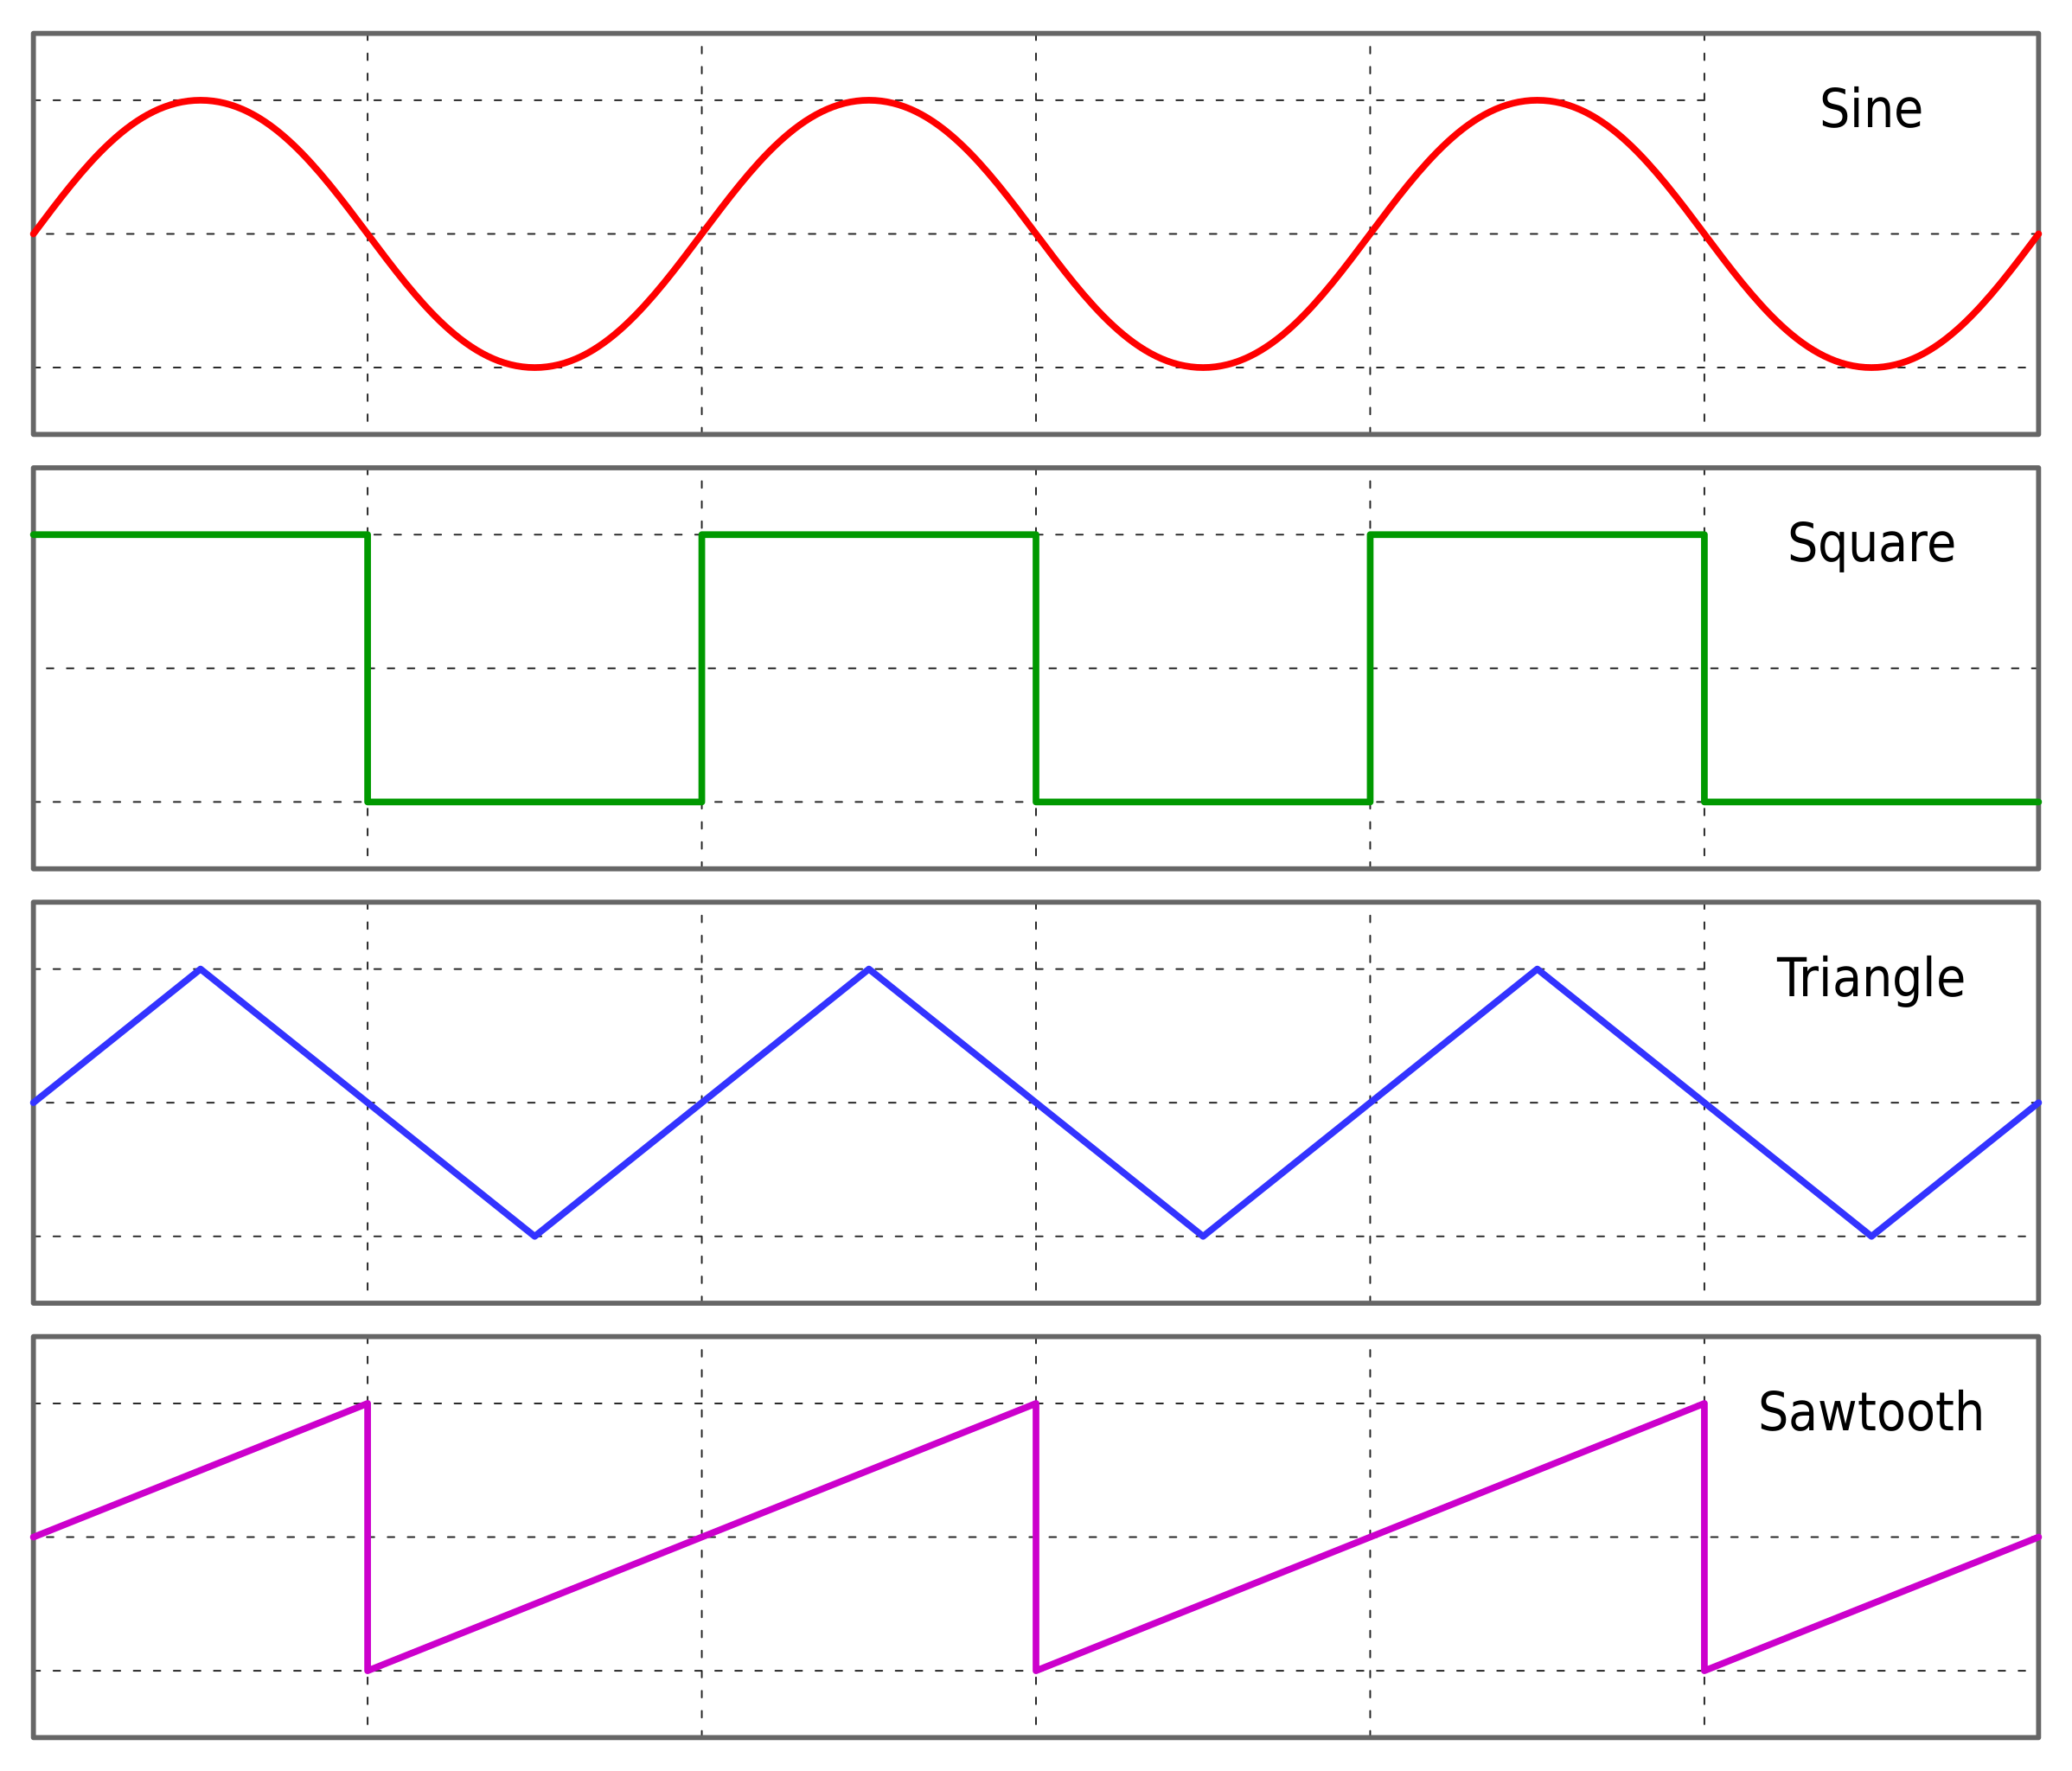
\includegraphics[width=0.8\textwidth]{assets/chap_2/wave_type.png}
\end{minipage}
\hfill
\begin{minipage}[c]{0.55\textwidth}
    \begin{itemize}
        \item Sine $\rightarrow$ period of $2\pi$.
        \item Square wave.
        \item Triangular wave.
        \item Sawtooth wave.
    \end{itemize}
\end{minipage}
\end{center}

\subsection{Quantization and Sampling}

\noindent
Để truyền dữ liệu (transmit data) qua môi trường chuyển dẫn (transmission medium), tín hiệu phải được:

\begin{itemize}
    \item converted ($\rightarrow$ quantization (lượng hóa)) $\Rightarrow$ chuyển đổi một dãy giá trị liên tục vào một cái gì đó cố định hơn $\Rightarrow$ continuous values (giá trị liên tục) $\rightarrow$ cần quantization.
    \item measured ($\rightarrow$ sampling (lấy mẫu)) $\Rightarrow$ đo tín hiệu tại các thời điểm khác nhau $\Rightarrow$ discrete time (thời gian rời rạc) $\rightarrow$ cần sampling.
\end{itemize}

\begin{itemize}
    \item[$\Rightarrow$] Máy tính lưu dữ liệu bằng các bit (0 và 1); nó cần một danh sách các con số cố định để lựa chọn $\Rightarrow$ cần quantization để chuyển tín hiệu liên tục thành tín hiệu rời rạc để lựa chọn (ví dụ: cân đồ nhưng kim nằm giữa 1kg và 1.1kg, nhưng mình không thể đọc được cái con số siêu lẻ $\rightarrow$ đọc 1kg luôn).
    \item[$\Rightarrow$] Máy tính không thể lưu trữ vô hạn trong một khoảng khắc nào đó, nếu nó làm thế thì sẽ dễ bị đầy bộ nhớ $\Rightarrow$ cần sampling để đo tín hiệu tại các thời điểm khác nhau $\rightarrow$ biến thời gian liên tục thành thời gian rời rạc để xử lý (ví dụ: quay video ở 30fps thay vì vô hạn fps).
\end{itemize}

\subsection{Sampling, Quantization, and Coding}

\noindent
\underline{Target:} chuyển tín hiệu analog sang digital representation.
\medskip

\noindent
Sampling and quantization:

\begin{itemize}
    \item Periodic measurement (đo đạt có chu kì) $\rightarrow$ sampling $\Rightarrow$ xử lý việc tín hiệu biến thiên liên tục theo thời gian bằng cách đo ngắt quãng.
    \item Dividing signal range (chia nhỏ dài tín hiệu) $\rightarrow$ quantization $\Rightarrow$ xử lý việc biên độ tín hiệu liên tục bằng cách chia nhỏ thành các khoảng (intervals) và gán giá trị cho chúng.
\end{itemize}
\medskip

\noindent
Coding (mã hóa):
\medskip

\noindent
$\rightarrow$ Focus on translating to binary $\Rightarrow$ gán một mã nhị phân (binary code) cho từng khoảng lượng tử hóa (quantization intervals).
\medskip

\begin{figure}[ht]
    \centering
    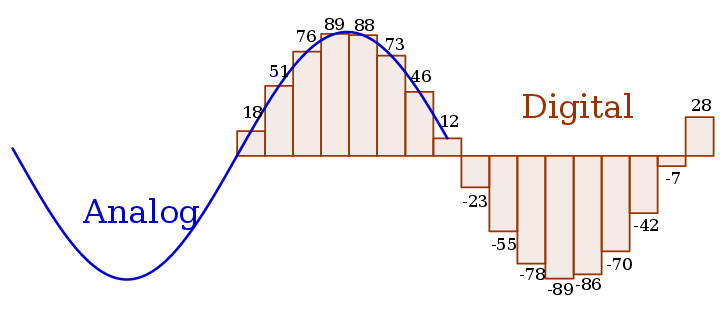
\includegraphics[width=0.5\textwidth]{assets/chap_2/sampling_coding.jpg}
\end{figure}
\medskip

\noindent
\textbf{Giải thích hình:}

\begin{itemize}
    \item Đường cong analog $\rightarrow$ tín hiệu thực tế; giá trị liên tục (continuous values).
    \item Các cột digital $\rightarrow$ dữ liệu máy tính ghi lại được $\Rightarrow$ mỗi cột đại diện cho một lần lấy mẫu (sampling).
    \item Các con số trên đỉnh mỗi cột $\rightarrow$ kết quả của lượng tử hóa (quantization).
\end{itemize}

\subsection{Symbol Rate}

\noindent
\underline{Self-note:} symbol rate nghĩa là tốc độ kí hiệu (định nghĩa ở mục tiếp theo).
\medskip

\begin{figure}[ht]
    \centering
    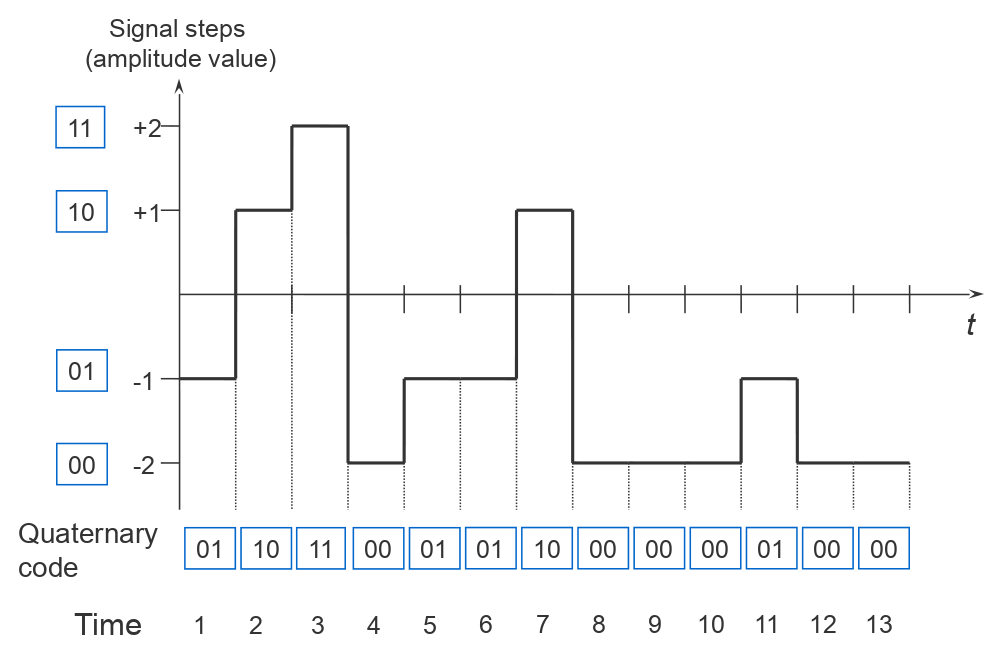
\includegraphics[width=0.55\textwidth]{assets/chap_2/sym_rate.png}
\end{figure}
\medskip

\noindent
$\rightarrow$ Biểu đồ minh họa quaternary (hệ tứ phân; nghĩa là có 4 trạng thái).

\begin{itemize}
    \item Amplitude value (giá trị biên độ) $\rightarrow$ tín hiệu không chỉ có 2 mức (0 và 1), mà có 4 mức điện áp khác nhau.
    \item Time $\rightarrow$ mỗi vạch là một khoảng thời gian cho một symbol.
\end{itemize}

\sidebox[-4.8cm]{Bonus:}{
$n$ (number of discrete values) $\rightarrow$ số lượng mức giá trị khác nhau mà tín hiệu có thể nhận được.

\begin{itemize}
    \item $n = 2 \rightarrow$ binary $\Rightarrow$ tín hiệu có 2 mức $\rightarrow$ chỉ được gửi 1 bit mỗi lần ($\log_2 2 = 1$).
    \item $n = 3 \rightarrow$ ternary $\Rightarrow$ tín hiệu có 3 mức.
    \item $n = 4 \rightarrow$ quaternary $\Rightarrow$ tín hiệu có 4 mức $\rightarrow$ chỉ được gửi 2 bit mỗi lần ($\log_2 4 = 2$).
    \item $n = 8 \rightarrow$ octonary $\Rightarrow$ tín hiệu có 8 mức $\rightarrow$ chỉ được gửi 3 bit mỗi lần ($\log_2 8 = 3$).
    \item $n = 10 \rightarrow$ denary $\Rightarrow$ tín hiệu có 10 mức.
\end{itemize}
}

\subsection{Bit Rate and Symbol Rate}

\noindent
Bit rate (tốc độ bit) $\rightarrow$ tổng số lượng các bit (0 và 1) được truyền đi trong một đơn vị thời gian (thường là giây) $\Rightarrow$ đơn vị là \textbf{bps} (bits per second).

$\Rightarrow$ Đây là tốc độ thực tế người ta quan tâm (tải file nhanh hay chậm phụ thuộc vào bit rate).
\medskip

\noindent
Symbol rate (tốc độ kí hiệu) $\rightarrow$ số lượng các kí hiệu (symbols) được truyền đi trong một đơn vị thời gian; một symbol là một trạng thái cụ thể của tín hiệu (ví dụ: một điện áp +5V, một xung sóng); đơn vị là \textbf{baud} (symbols per second).

$\Rightarrow$ Đây là tốc độ làm việc của phần cứng (chẳng hạn như dây cáp phải đổi state (trạng thái) bao nhiêu lần).
\medskip

\noindent
The ratio between bit rate and symbol rate $\rightarrow$ phụ thuộc vào công nghệ mã hóa đường truyền (line encoding scheme) được sử dụng.
\medskip

\sidebox[-4cm]{Self-note:}{Line code $\rightarrow$ là quy tắt để máy tính truyền tín hiệu lên dây dẫn sao cho bên nhận có thể hiểu được.}

$\Rightarrow$ Quy định: số lượng tín hiệu tối đa có thể truyền qua transmission media được sử dụng (số 1 thì điện áp như nào, số 0 thì điện áp như nào); xác định bởi layer protocol được sử dụng.
\medskip

\begin{figure}[ht]
    \centering
    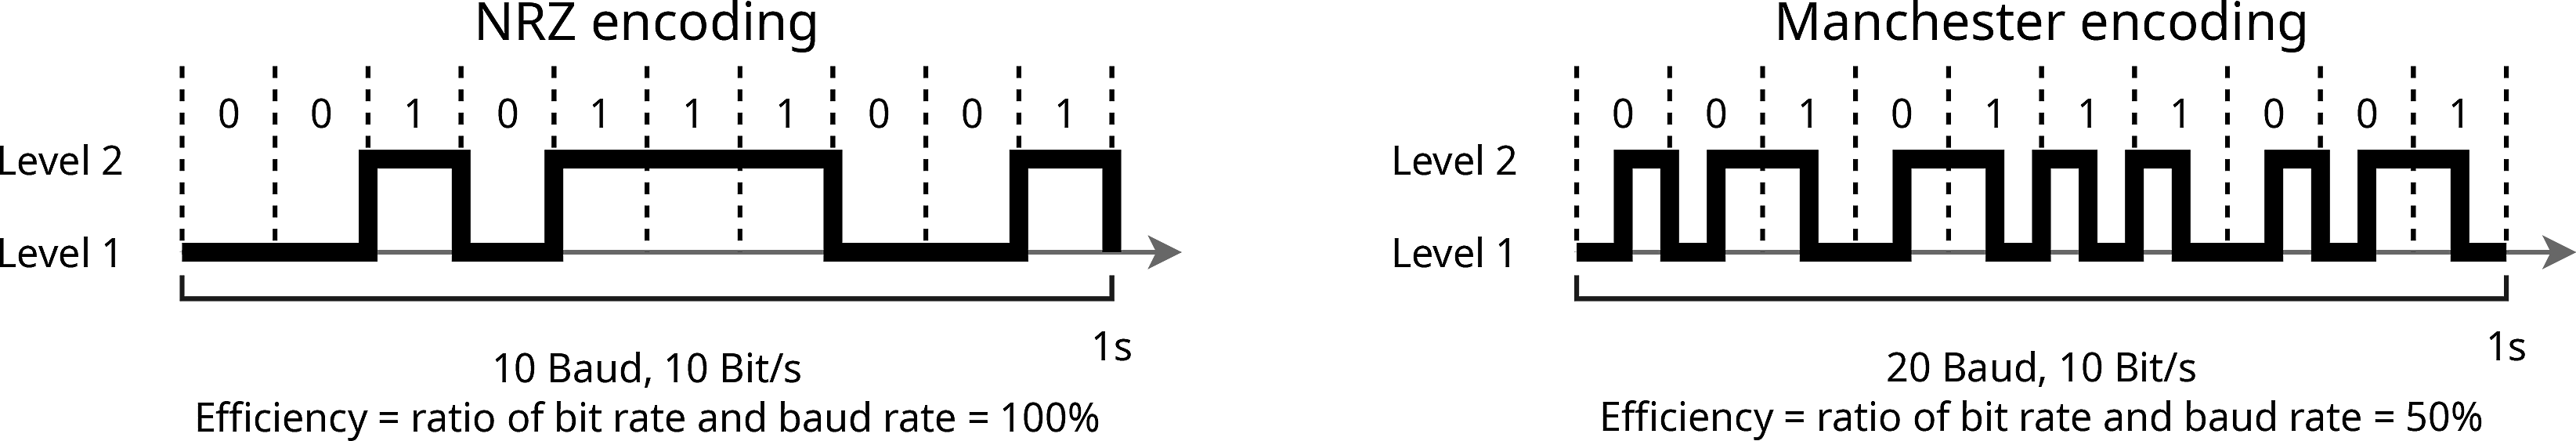
\includegraphics[width=1\textwidth]{assets/chap_2/line_code_ex.png}
\end{figure}

\sidebox[-6cm]{Bonus:}{
\noindent
NRZ (Non-Return to Zero) encoding $\rightarrow$ gặp số 0 thì giữ điện áp mức thấp, còn gặp 1 thì giữ ở mức cao.
\medskip

\noindent
Manchester Encoding $\rightarrow$ không quan tâm mức cao hay thấp, chỉ quan tâm đến sự thay đổi (transition) giữa bit:

\begin{itemize}
    \item Số 0 $\rightarrow$ đang cao nhảy xuống thấp (falling edge).
    \item Số 1 $\rightarrow$ đang thấp nhảy lên cao (rising edge).
\end{itemize}
\medskip
}

\subsection{Data Rate}

\noindent
Data rate $\rightarrow$ tốc độ truyền dữ liệu tối đa mà đường truyền có thể tải được.

$\Rightarrow$ Nó trả lời cho câu "trong 1s thì gửi được bao nhiêu bit đi?".
\medskip

\noindent
\textbf{$\rightarrow$ Hai yếu tố ảnh hưởng:}

\begin{enumerate}
    \item Bandwidth (băng thông), kí hiệu: $H$ $\rightarrow$ độ rộng của đường vận chuyển. Đường càng rộng (Hertz càng cao) $\Rightarrow$ bit chạy càng nhiều.
    \item Levels (mức tín hiệu) (hoặc độ nhiễu (noise)), kí hiệu: $V$ $\rightarrow$ nếu không có nhiễu $\Rightarrow$ dùng càng nhiều mức tín hiệu ($V$ càng cao; như 4 mức, 8 mức), tốc độ càng nhanh.
\end{enumerate}

\begin{mybox}{Định luật Hartley}
\begin{equation*}
    \text{Maximum data rate [bit/s]} = 2 * H * \log_2(V)
\end{equation*}
\end{mybox}

\noindent
Trong đó:

\begin{itemize}
    \item $H \rightarrow$ độ rộng băng tần của đường truyền (tính bằng Hz) $\Rightarrow$ Đường càng rộng thì chạy càng nhanh.
    \item $V \rightarrow$ số lượng mức tín hiệu (như $n = 2$, $n = 4$).
\end{itemize}
\medskip

\sidebox[-5.5cm]{Note:}{Định luật của Hartley là \textbf{điều kiện lý tưởng} $\rightarrow$ đường truyền hoàn hảo, không có nhiễu (noiseless) $\Rightarrow$ tốc độ tối đa phụ thuộc vào việc mình tạo ra được bao nhiêu tín hiệu.}

\subsection{Ideal vs. Real Transmission}

\begin{figure}[ht]
    \centering
    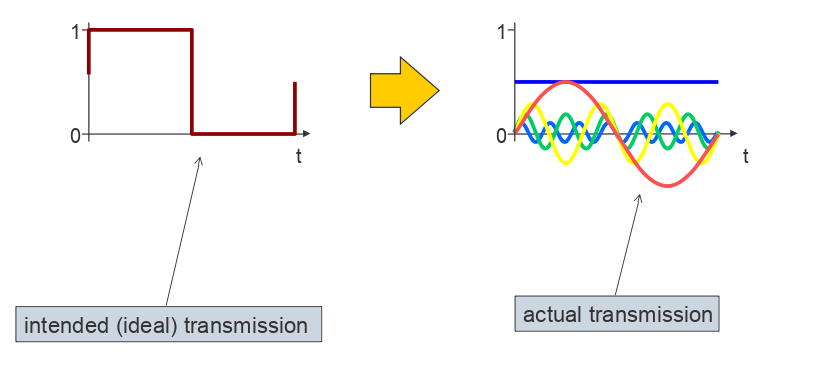
\includegraphics[width=0.75\textwidth]{assets/chap_2/ideal_vs_real.png}
\end{figure}
\medspace

\noindent
Giải thích:

\begin{itemize}
    \item Bên lý tưởng $\rightarrow$ tín hiệu hoàn hảo mà máy tính gửi đi dưới dạng sóng vuông (square wave) $\Rightarrow$ không bị nhiễu, chuyển đổi tức thì từ mức 0 lên 1.
    \item Bên thực tế $\rightarrow$ tín hiệu bị biến thành sóng do bị nhiễu, cộng thêm các đường sóng nhỏ (màu xanh, vàng) (theo như chuỗi Fourier (Fourier series) $\rightarrow$ một sóng vuông thực tế là tổng hợp của vô số sóng hình sin có tần số khác nhau cộng lại) $\Rightarrow$ tín hiệu không chuyển đổi tức thì từ mức 0 lên 1 mà cần thời gian để chuyển đổi.
\end{itemize}

\noindent
$\Rightarrow$ Nếu đường truyền quá dài hoặc quá tệ (do bị nhiễu quá nhiều chẳng hạn) $\rightarrow$ sóng sẽ bị "méo" đến mức máy tính không thể phân biệt được đâu là mức 1, đâu là mức 0 nữa.
\medskip

\noindent
$\rightarrow$ Ở mặt lý tưởng, Claude Shannon cho rằng mục tiêu của truyền tin là tái tạo lại chính xác thông tin $\rightarrow$ tuy nhiên, trên thực tế, có rất nhiều yếu tố làm suy giảm tín hiệu trong quá trình truyền dẫn.
\medskip

\subsection{Attenuation}

\noindent
Attenuation (suy hao) $\rightarrow$ tín hiệu yếu đi khi truyền xa.

$\rightarrow$ Làm cho suy yếu tín hiệu (signal weakening) $\rightarrow$ làm yếu đi biên độ của tín hiệu ngày càng nhiều, theo quãng đường truyền tin của các phương tiện truyền tải $\Rightarrow$ năng lượng tín hiệu mất dần.
\medskip

\noindent
\textbf{$\rightarrow$ Hậu quả:} nếu biên độ (amplitude) của tín hiệu quá thấp so với mức yêu cầu $\Rightarrow$ máy sẽ không thể nhận biết được tín hiệu nữa $\Rightarrow$ mất dữ liệu.

$\Rightarrow$ Attenuation giới hạn khoảng cách tối đa có thể truyền tải tín hiệu với mọi transmission media.
\medskip

\noindent
\textbf{Quy luật:} Tần số càng cao, suy hao càng lớn.
\medskip

\sidebox[-3.7cm]{Idea:}{Người ta có thể khắc phục điều này bằng việc sử dụng repeater (bộ lặp) hoặc amplifier (bộ khuếch đại) để tăng cường tín hiệu, để tín hiệu có thể truyền đi tiếp.}

\subsection{Noise and Distortion}

\noindent
\textbf{Noise} (nhiễu) $\rightarrow$ tín hiệu không mong muốn làm thay đổi tín hiệu gốc.

\begin{itemize}
    \item Thermal noise (nhiễu nhiệt) $\rightarrow$ do chuyển động ngẫu nhiên của các electron trong dây dẫn tạo ra.
    \item Intermodulation noise (nhiễu tương hỗ) $\rightarrow$ do các tần số không mong muốn kết hợp với tín hiệu ban đầu.
    \item Crosstalk (nhiễu chéo) $\rightarrow$ do tín hiệu từ dây dẫn khác truyền sang.
    \item Impulse noise (nhiễu xung) $\rightarrow$ do các sự kiện đột ngột như sét đánh hoặc các sự cố điện.
\end{itemize}
\medskip

\noindent
\textbf{Distortion} (biến dạng) $\rightarrow$ tín hiệu bị thay đổi hình dạng do các đặc tính của phương tiện truyền dẫn.

\begin{itemize}
    \item Echoes (tiếng vang) $\rightarrow$ tín hiệu phản xạ trở lại.
    \item Extreme low frequency (ELF) (tần số cực thấp) $\rightarrow$ tín hiệu tần số thấp bị suy giảm nhiều hơn.
    \item Delay distortion (biến dạng trễ) $\rightarrow$ các thành phần tần số khác nhau truyền với tốc độ khác nhau.
\end{itemize}
\medskip

\noindent
$\rightarrow$ Plus attenuation, refraction (làm lệch hướng), reflection (phản xạ), etc.

\noindent
\begin{center}
\begin{minipage}[c]{0.4\textwidth}
    \centering
    
\includegraphics[width=0.7\textwidth]{assets/chap_2/gauss.png}
\end{minipage}
\hfill
\begin{minipage}[c]{0.55\textwidth}
    AWGN (Additive White Gaussian Noise) $\rightarrow$ mô hình nhiễu phổ biến nhất.
\end{minipage}
\end{center}

\noindent
\textbf{Giải thích:}

\begin{itemize}
    \item Additive (cộng tính) $\rightarrow$ nhiễu được thêm vào tín hiệu gốc.
    \item White $\rightarrow$ phổ tần số rộng (giống như ánh sáng trắng) $\Rightarrow$ nhiễu trắng chứa tất cả các tần số với công suất bằng nhau.
    \item Gaussian Noise (nhiễu Gauss) $\rightarrow$ cường độ nhiễu tuân theo phân phối Gaussian (phân phối chuẩn - hình chuông).
\end{itemize}
\medskip

\noindent
\textbf{Gaussian channel} (kênh Gauss) $\rightarrow$ khi một kênh truyền (đường dây) chịu tác động chủ yếu của loại nhiễu này (nhiễu nhiệt, bức xạ nền, ...).
\medskip

\subsection{Bit Error Rate (BER)}

\noindent
Bit Error Rate (Tỷ lệ lỗi bit) $\rightarrow$ đánh giá độ tin cậy của một đường truyền dữ liệu.

$\Rightarrow$ Nhiễu có thể làm suy giảm chất lượng đường truyền $\rightarrow$ có thể khiến máy tính khi nhận đọc sai (như 0 thành 1, hay 1 thành 0 chẳng hạn).
\medskip

\noindent
$\Rightarrow$ BER được tính theo tỉ lệ phần trăm các bit bị sai so với tổng số bit đã được truyền đi.
\medskip

\begin{mybox}{Bit Error Rate}
\begin{equation*}
    \text{BER} = \frac{\text{Number of erroneous bits (số bit bị lỗi)}}{\text{Number of transmitted bits (tổng số bit đã truyền)}}
\end{equation*}
\end{mybox}

\noindent
\textbf{Ví dụ:} gửi 1.000 bit và có 1 bit bị sai $\Rightarrow$ BER = $\frac{1}{1000} = 0.001$ (hay $10^{-3}$).

\vspace{0.5cm}

\noindent
Typical BER values for different link types:

\begin{itemize}
    \item POTS (Plain Old Telephone Service) $\rightarrow$ $2*10^{-4}$.
    \item Radio links $\rightarrow$ $10^{-3}$ to $10^{-4}$.
    \item Ethernet $\rightarrow$ $10^{-9}$ to $10^{-10}$.
    \item Fiber (cáp quang) $\rightarrow$ $10^{-10}$ to $10^{-12}$.
\end{itemize}
\medskip

\sidebox[-10cm]{Self-note:}{
$\rightarrow$ Mạng radio có BER tệ nhất $\Rightarrow$ do chịu nhiều tác động từ môi trường xung quanh như thời tiết, vật cản, ... $\Rightarrow$ dễ bị nhiễu hơn so với mạng dây (như Ethernet hay fiber).
\medskip

\noindent
BER \textbf{càng nhỏ} (số có mũ càng âm lớn) $\Rightarrow$ đường truyền \textbf{càng tốt}.
}

\sidebox[-4cm]{Bonus:}{Giảm BER $\rightarrow$ tăng cường độ tín hiệu để át nhiễu.
\medskip

\noindent
$\Rightarrow$ Việc này có thể gây tốn kém (như tốn điện do phải tăng biên độ $\rightarrow$ tăng mức tiêu thụ năng lượng), và gây nhiễu cho các thiết bị xung quanh.
}

\subsection{Data Rate on a Noisy Channel}

\noindent
$\rightarrow$ Mọi kênh truyền thực tế đều bị nhiễm bởi nhiễu.
\medskip

\noindent
$\rightarrow$ Tốc độ truyền không chỉ phụ thuộc vào số mức tín hiệu ($V$), mà còn phụ thuộc vào cường độ tín hiệu mạnh hơn nhiễu bao nhiêu lần.

$\Rightarrow$ Signal-to-Noise Ratio (SNR) $\rightarrow$ tỉ lệ công suất tín hiệu ($S$) và công suất nhiễu ($N$).
\medskip

\begin{mybox}{Signal-to-Noise Ratio}
\begin{equation*}
    \text{SNR} = \frac{\text{Signal Power }(S)}{\text{Noise Power }(N)}
\end{equation*}
\end{mybox}

\noindent
$\Rightarrow$ SNR càng cao $\Rightarrow$ tín hiệu càng mạnh hơn nhiễu.
\medskip

\noindent
\textbf{Ví dụ:} nói chuyện trong một quán karaoke, giọng mình ($S$) so với tiếng nhạc ồn ($N$), nếu $S < N$, người ta sẽ không nghe được mình nói gì cả $\rightarrow$ tốc độ truyền tin $= 0$.
\medskip

\begin{mybox}{Shannon-Hartley theorem}
\begin{equation*}
    \text{Maximum data rate [bit/s]} = H * \log_2(1 + \frac{S}{N})
\end{equation*}
\end{mybox}

\noindent
Trong đó:

\begin{itemize}
    \item Signal strength ($S$) $\rightarrow$ cường độ tín hiệu.
    \item Noise strength ($N$) $\rightarrow$ cường độ nhiễu.
    \item Bandwidth ($H$) $\rightarrow$ độ rộng băng tần (tính bằng Hz).
\end{itemize}
\medskip

\noindent
The SNR is commonly expressed in decibel (dB):

\begin{equation*}
    \text{SNR [dB]} = 10 * \log_{10}(\frac{S}{N})
\end{equation*}
\medskip

\noindent
\textbf{Finalize:} định lý Shannon-Hartley cho ta biết giới hạn lý thuyết về tốc độ truyền dữ liệu tối đa trên một kênh truyền có nhiễu.
\medskip

\sidebox[-6cm]{Self-note:}{
Công thức Shannon ở trên dùng tỷ số thường ($S/N$) $\rightarrow$ nếu đề bài cho SNR là 30dB, mình \textbf{không được} thay số 30 vào công thức Shannon
\medskip

\noindent
$\Rightarrow$ Phải chuyển đổi 30dB thành 1000 lần ($S/N = 10^{30/10} = 10^3 = 1000$) rồi mới thay vào công thức Shannon.
}

\section{Data Encoding}

\subsection{Line Encoding}

\subsubsection{Baseband and Broadband (part 1)}

\noindent
Vấn đề được đặt ra: làm thế nào để có thể đưa các bit (0 và 1) lên đường truyền?

$\rightarrow$ Data encoding (mã hóa dữ liệu) cần xác định được kí hiệu nào là 0, kí hiệu nào là 1.
\medskip

\noindent
\underline{Therefore}:

\textbf{$\rightarrow$ Baseband} (dải cơ sở) $\rightarrow$ truyền tín hiệu nguyên bản (transmitted as is); tín hiệu số (xung vuông) được đẩy trực tiếp lên dây $\Rightarrow$ cần có data encoding để quy định rõ các mức điện áp 0 hay 1 $\rightarrow$ thường dùng cho mạng LAN hoặc kết nối ngắn.
\medskip

\subsubsection{Encoding Schemes}

\noindent
Cơ chế mã hóa (encoding schemes) $\rightarrow$ tập hợp các quy tắc để chuyển đổi các bit (0 và 1) thành các tín hiệu vật lý để truyền.
\medskip

\noindent
\textbf{Có 3 yếu tố chính:}

\begin{itemize}
    \item Robust (bền vững) $\rightarrow$ tín hiệu phải đủ mạnh và rõ ràng để chống lại nhiễu và distortion (biến dạng) $\rightarrow$ cho dù bị biến đổi thì bên nhận vẫn đọc được đâu là 0, đâu là 1.
    \item Efficient (hiệu quả) $\rightarrow$ mục tiêu: đạt được tốc độ truyền dữ liệu cao nhất có thể $\Rightarrow$ cơ chế nào cho phép truyền nhiều bit nhất trong cùng một khoảng thời gian (hoặc cùng dải tần) thì hiệu quả nhất.
    \item Synchronous (đồng bộ) $\rightarrow$ máy gửi và máy nhận phải cùng "nhịp" với nhau thì mới biết được khi nào một bit bắt đầu và kết thúc.
\end{itemize}

\clearpage

\noindent
Cách cách để đồng bộ hóa:

\begin{itemize}
    \item Dùng explicit clock signal (tín hiệu xung nhịp rõ ràng) $\rightarrow$ gửi một tín hiệu xung nhịp riêng biệt cùng với dữ liệu $\Rightarrow$ tốn kém.
    \item Synchronize on certain points (đồng bộ theo thời điểm) $\rightarrow$ sử dụng như "start bit" để báo hiệu bắt đầu.
    \item Self-synchronizing signal (tự đồng bộ) $\rightarrow$ bản thân tín hiệu luôn chứa thông tin về xung nhịp (nhờ việc đảo chiều liên tục) $\Rightarrow$ máy nhận không bao giờ lạc nhịp (như Manchester encoding).
\end{itemize}

\noindent
$\rightarrow$ There are many ways to encode binary data onto a line; many different encodings are used in different technologies.
\medskip

\subsubsection{Non-Return-to-Zero (NRZ)}

\begin{figure}[htbp]
    \centering
    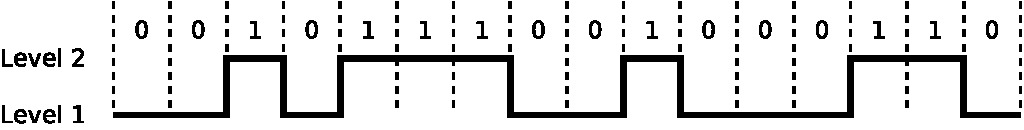
\includegraphics[width=1\textwidth]{assets/chap_2/nrz.jpg}
\end{figure}
\medskip

\noindent
$\rightarrow$ là kĩ thuật mã hóa đường truyền đơn giản nhất.
\medskip

\noindent
\textbf{Nguyên lý hoạt động:} NRZ thực hiện việc gán mức điện áp trực tiếp cho các bit:

\begin{itemize}
    \item Bit 0 $\rightarrow$ được mã hóa bằng mức điện áp thấp (level 1, chẳng hạn như -5V).
    \item Bit 1 $\rightarrow$ được mã hóa bằng mức điện áp cao (level 2, chẳng hạn như +5V).
\end{itemize}
\medskip

\noindent
Lý do gọi là "Non-Return-to-Zero" $\rightarrow$ trong suốt thời gian truyền một bit (ví dụ như bit 1) $\rightarrow$ điện áp giữ nguyên ở mức cao từ đầu đến cuối $\Rightarrow$ không trở về mức 0 (zero) giữa các bit (khác với mã RZ).

$\rightarrow$ Khác với mã RZ (Return-to-Zero) $\rightarrow$ nếu là bit 1 (mức cao), điện áp nhảy lên mức cao $\Rightarrow$ nhưng bắt buộc phải trở về mức 0 trước khi bit tiếp theo bắt đầu (khi đi được nửa thời gian của bit đó).
\medskip

\begin{itemize}
    \item \textbf{Pros:} đơn giản và hiệu quả (simple and efficient) $\rightarrow$ sử dụng băng thông rất tốt do tần số tín hiệu không phải thay đổi quá nhanh (so với lại Manchester encoding).
    \item \textbf{Cons:} gặp rắc rối lớn khi truyền dữ liệu có một chuỗi dài các bit giống nhau (như đã nói ở trên) $\Rightarrow$ đường tín hiệu sẽ \textbf{gặp 2 lỗi}: clock recovery (máy sẽ không nhận biết mình đang ở bit thứ mấy) và baseline wander (giữ điện áp quá lâu có thể bị thay đổi mức điện áp trung bình $\Rightarrow$ máy thu sẽ không biết đâu là mức cao, đâu là mức thấp nữa).
\end{itemize}

\sidebox[-5cm]{Bonus:}{
$\rightarrow$ Kĩ thuật này được sử dụng trong CAN bus system (Controller Area Network) $\rightarrow$ một hệ thống dùng để kết nối với các bộ điều khiển trong xe hơi do Bosch phát triển từ những năm 1980.
}

\subsubsection{Manchester Code}

\begin{figure}[H]
    \centering
    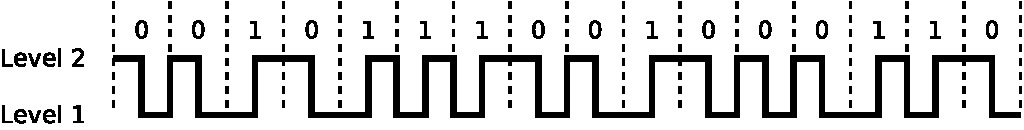
\includegraphics[width=1\textwidth]{assets/chap_2/man_code.jpg}
\end{figure}
\medskip

\noindent
$\rightarrow$ là kĩ thuật giải quyết cho vấn đề đồng bộ hóa.

$\Rightarrow$ Tập trung vào hướng di chuyển (transition) của dòng điện ở giữa khoảng thời gian mỗi bit (khác với NRZ chỉ quan tâm đến điện áp cao hay thấp).

\begin{itemize}
    \item Logical 1 $\rightarrow$ encoded with a rising edge (sườn lên) $\Rightarrow$ thay đổi từ signal level 1 (mức thấp) sang signal level 2 (mức cao).
    \item Logical 0 $\rightarrow$ encoded with a falling edge (sườn xuống) $\Rightarrow$ thay đổi từ signal level 2 (mức cao) sang signal level 1 (mức thấp).
\end{itemize}
\medskip

\noindent
\textbf{$\rightarrow$ Quy tắc đặt biệt:} nếu có 2 bit giống nhau đi liền (ví dụ: \texttt{0} và \texttt{0} ở sát nhau), thì tại cuối bit thứ nhất, tín hiệu sẽ phải đổi trạng thái để phân biệt cho việc đổi trạng thái của bit sau.
\medskip

\begin{itemize}
    \item \textbf{Pros:} tự đồng bộ (self-synchronizing) $\rightarrow$ do ở chính giữa của mỗi bit luôn có một transition $\Rightarrow$ máy nhận có thể dùng cái này để đếm xung (clock) $\Rightarrow$ không bao giờ bị nhầm lẫn giữa các bit dù có gửi cả chuỗi bit giống nhau dài cách mấy.
    \item \textbf{Cons:} hiệu suất thấp, chỉ đạt cỡ 50\% so với NRZ $\Rightarrow$ vì khi 1 bit được gửi $\rightarrow$ tín hiệu phải thay đổi trạng thái tới 2 lần (nửa đầu khác, nửa sau khác) $\Rightarrow$ tốc độ Baud phải gấp đôi so với tốc dộ bit $\rightarrow$ tốn băng thông hơn so với NRZ.
\end{itemize}

\sidebox[-10cm]{Self-note:}{
$\Rightarrow$ Nếu quan sát kĩ trên hình vẽ thì Manschester encoding sẽ luôn có một transition ở giữa bit; nửa trái là để phân biệt giữa 2 bit, nửa phải là để biểu diễn giá trị của bit đó (0 hay 1 thông qua mức thấp hay cao).
}

\sidebox[-4cm]{Bonus:}{
$\rightarrow$ Do tính ổn định và khả năng tự đồng bộ cao, mã này được sử dụng trong mạng Ethernet 10 Mbps (10BASE-T hay 10BASE2).
}

\subsection{Modulation}

\subsubsection{Baseband and Broadband (part 2)}

\noindent
Vấn đề được đặt ra: làm thế nào để truyền dữ liệu đi xa hơn và truyền được nhiều luồng dữ liệu cùng một lúc?

$\rightarrow$ Modulation (biến đổi tín hiệu) $\rightarrow$ biến đổi digital signal thành analog signal trước khi truyền $\Rightarrow$ by using different carrier signals (frequencies) $\rightarrow$ several transmissions can happen simultaneously.
\medskip

\noindent
\underline{Therefore}:

\textbf{$\rightarrow$ Broadband} (dải rộng) $\rightarrow$ tín hiệu số được biến đổi (modulate) thành analog trước khi truyền $\Rightarrow$ cho phép chia đường truyền thành nhiều kênh tần số khác nhau (nhiều luồng dữ liệu có thể truyền cùng một lúc) $\rightarrow$ dùng cho truyền dẫn quãng dài như truyền hình cáp hay 4G chẳng hạn.
\medskip

\clearpage

\subsubsection{Principle of Modulation}

\begin{mybox}{Electromagnetic Signal (tín hiệu điện tử)}
\begin{equation*}
    s(t) = A * \sin(2 \pi f t + \phi)
\end{equation*}
\end{mybox}

\noindent
Trong đó:

\begin{itemize}
    \item $A$ $\rightarrow$ amplitude (biên độ).
    \item $f$ $\rightarrow$ frequency (tần số).
    \item $\phi$ $\rightarrow$ phase (pha).
    \item $t$ $\rightarrow$ time (thời gian).
\end{itemize}

\begin{figure}[ht]
    \centering
    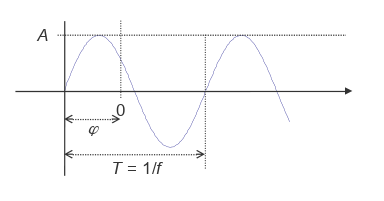
\includegraphics[width=0.8\textwidth]{assets/chap_2/electro_mag_wave.png}
\end{figure}
\medskip

\noindent
$\Rightarrow$ Dữ liệu đã được biến đổi thành tần số mang (carrier frequency) $\rightarrow$ có thể truyền đi xa hơn và nhiều luồng dữ liệu có thể truyền cùng lúc.
\medskip

\begin{figure}[ht]
    \centering
    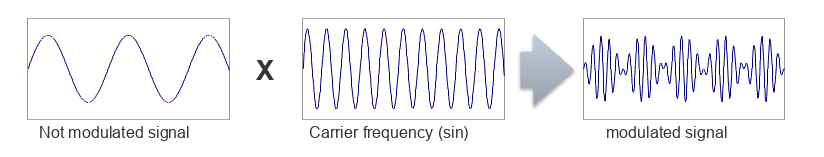
\includegraphics[width=1\textwidth]{assets/chap_2/modem_illust.png}
\end{figure}
\medskip

\noindent
$\rightarrow$ \textbf{Modem:} \textbf{Mo}dulation-\textbf{Dem}odulation process (quá trình biến đổi và giải biến đổi).
\medskip

\subsubsection{Amplitude Shift Keying (ASK)}

\noindent
ASK: điều chế dịch biên độ (hoặc gọi là điều chế biên độ cũng được).
\medskip

\noindent
$\rightarrow$ Là phương pháp điều chế cơ bản được sử dụng trong broadband (phương pháp thứ nhất).

$\Rightarrow$ Nơi dữ liệu được mã hóa bằng cách \textbf{thay đổi biên độ} (amplitude) của sóng mang điện từ.
\medskip

\begin{figure}[H]
    \centering
    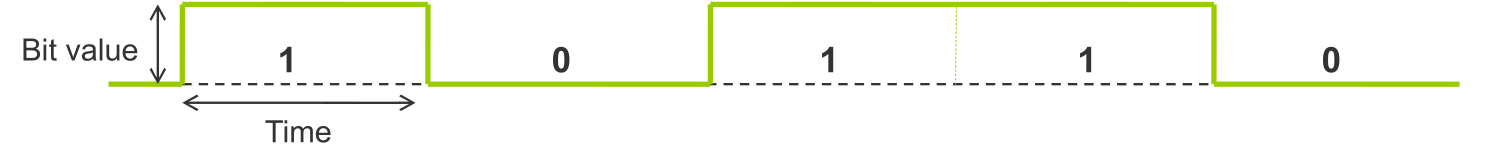
\includegraphics[width=1\textwidth]{assets/chap_2/bit_illust.png}
\end{figure}
\medskip

\noindent
Amplitude Modulation (discrete, Amplitude Shift Keying - ASK) $\rightarrow$ biến đổi biên độ $\Rightarrow$ kí hiệu $A$ từ công thức trên.

\begin{figure}[H]
    \centering
    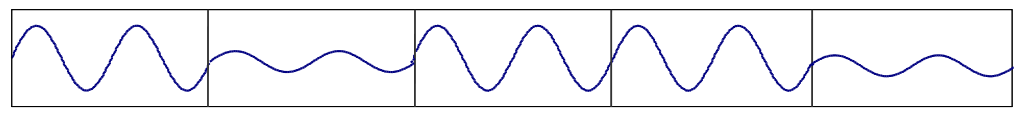
\includegraphics[width=1\textwidth]{assets/chap_2/ask_wave.png}
\end{figure}
\medskip

\noindent
\textbf{Nguyên lý hoạt động:}

\begin{itemize}
    \item Bit 1 $\rightarrow$ được mã hóa bằng một sóng có biên độ cao ($A_{high}$).
    \item Bit 0 $\rightarrow$ được mã hóa bằng một sóng có biên độ thấp ($A_{low}$).
\end{itemize}
\medskip

\noindent
$\rightarrow$ Máy phát sóng mạnh khi gửi bit 1, và yếu khi gửi bit 0.
\medskip

\begin{itemize}
    \item \textbf{Pros:} easy to realize (dễ thực hiện) $\Rightarrow$ chỉ cần thay đổi biên độ của sóng mang; giải mã ở cả 2 đầu máy phát và thu; does not need much bandwidth (không tốn nhiều băng thông) $\rightarrow$ do ASK thay đổi biên độ, tần số được giữ nguyên $\Rightarrow$ nó không tốn nhiều dải tần (so với FSK sẽ nói ở dưới).
    \item \textbf{Cons:} nhạy cảm với noise; attenuation và noise luôn làm thay đổi biên độ của tín hiệu trong môi trường thực tế $\rightarrow$ nếu gửi bit 1 (biên độ cao) nhưng quá nhiều yếu tố gây nhiễu thì máy sẽ đọc lộn thành bit 0 (biên độ thấp).
\end{itemize}
\medskip

\noindent
$\Rightarrow$ Do đó, ASK không được sử dụng rộng rãi cho truyền dữ liệu tốc độ cao, hay ở khoảng cách xa vì dễ gây ra lỗi bit (BER cao).
\medskip

\noindent
\textbf{Ứng dụng:} thường được sử dụng trong truyền dẫn quang (optical transmission) $\rightarrow$ low noise.
\medskip

\sidebox[-4cm]{Self-note:}{
$\rightarrow$ Cứ xem ASK như nhìn dãy đèn ở khoảng cách xa $\rightarrow$ đèn sáng (bit 1) và đèn tắt (bit 0) $\Rightarrow$ dễ thao tác, nhưng nếu trời bị sương mù dày đặc (nhiễu cao) $\rightarrow$ nhìn nhầm hoặc không thấy.
}

\subsubsection{Frequency Shift Keying (FSK)}

\noindent
FSK: điều chế dịch tần số (hoặc gọi là điều chế tần số cũng được).
\medskip

\noindent
$\rightarrow$ Là phương pháp điều chế sử dụng trong broadband (phương pháp thứ hai).

$\Rightarrow$ Nơi dữ liệu được mã hóa bằng cách \textbf{thay đổi tần số} (frequency) của sóng mang điện từ.
\medskip

\begin{figure}[htbp]
    \centering
    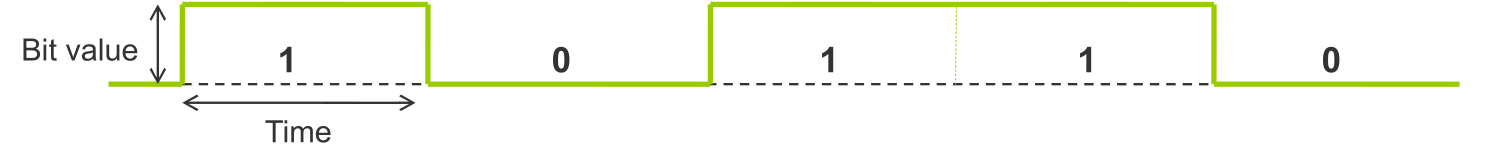
\includegraphics[width=1\textwidth]{assets/chap_2/bit_illust.png}
\end{figure}
\medskip

\noindent
Frequency Modulation (discrete, Frequency Shift Keying - FSK) $\rightarrow$ biến đổi tần số $\Rightarrow$ kí hiệu $f$ từ công thức trên.

\begin{figure}[ht]
    \centering
    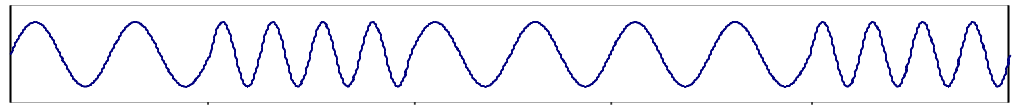
\includegraphics[width=1\textwidth]{assets/chap_2/fsk_wave.png}
\end{figure}
\medskip

\clearpage

\noindent
\textbf{Nguyên lý hoạt động:}

\begin{itemize}
    \item Bit 1 $\rightarrow$ được mã hóa bằng một sóng có tần số cao ($f_{high}$).
    \item Bit 0 $\rightarrow$ được mã hóa bằng một sóng có tần số thấp ($f_{low}$).
\end{itemize}

\noindent
$\rightarrow$ Máy phát sóng nhanh khi gửi bit 1, và chậm khi gửi bit 0.
\medskip

\begin{itemize}
    \item \textbf{Pros:} ít nhạy cảm với noise hơi ASK $\Rightarrow$ vì nhiễu thường làm thay đổi biên độ (độ cao) của sóng chứ không phải tần số (độ nhanh/chậm của sóng) $\Rightarrow$ tín hiệu ổn định hơn ASK.
    \item \textbf{Cons:} lãnh phí tần số (waste of frequencies) $\rightarrow$ cần dành riêng 2 khoảng tần số khác nhau cho bit 0 và bit 1; tốn nhiều băng thông (needs a lot of bandwidth) $\rightarrow$ do phải phân biệt rõ ràng giữa 2 tần số cao thấp $\Rightarrow$ 2 đứa đó nằm cách xa nhau, dẫn đến tốn nhiều tiết diện trên dải băng tần.
\end{itemize}

\noindent
$\rightarrow$ Do tốn nhiều băng thông $\Rightarrow$ ít được dùng cho các ứng dụng cần tốc độ cực cao, tuy nhiên độ bền (robustness) của nó uy tín.
\medskip

\noindent
\textbf{Ứng dụng:} nguyên lý ban đầu được dùng để truyền dữ liệu qua điện thoại (phone lines).
\medskip

\sidebox[-5cm]{Self-note:}{
\noindent
$\rightarrow$ Cứ xem FSK như giọng hát $\rightarrow$ nốt cao (bit 1) và nốt trầm (bit 0) $\Rightarrow$ dù có đang trong phòng ồn ào (bị noise) $\rightarrow$ vẫn phân biệt được nốt cao hay thấp (khó nhầm lẫn hơn so với ASK) $\rightarrow$ tuy nhiên, phải có quãng giọng rộng (được xem như cần nhiều bandwidth) mới có thể hát được cả 2 nốt này rõ ràng.
}

\subsubsection{Phase Shift Keying (PSK)}

\noindent
PSK: điều chế dịch pha (hoặc gọi là điều chế pha cũng được).
\medskip

\noindent
$\rightarrow$ Là phương pháp điều chế sử dụng trong broadband (phương pháp thứ ba).

$\Rightarrow$ Nơi dữ liệu được mã hóa bằng cách \textbf{thay đổi pha} ($\phi$ phase) của sóng mang điện từ.
\medskip

\begin{figure}[htbp]
    \centering
    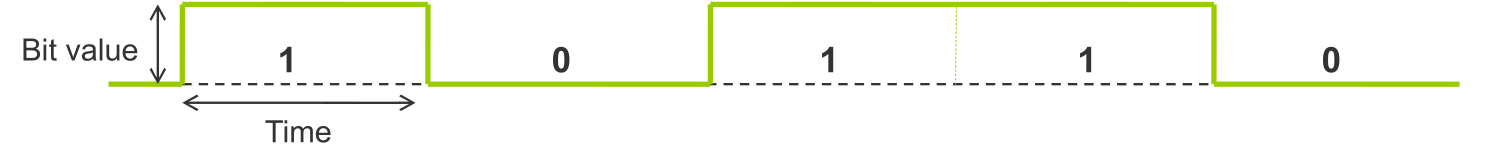
\includegraphics[width=1\textwidth]{assets/chap_2/bit_illust.png}
\end{figure}
\medskip

\noindent
Phase Modulation (discrete, Phase Shift Keying - PSK) $\rightarrow$ biến đổi pha $\Rightarrow$ kí hiệu $\phi$ từ công thức trên.

\begin{figure}[ht]
    \centering
    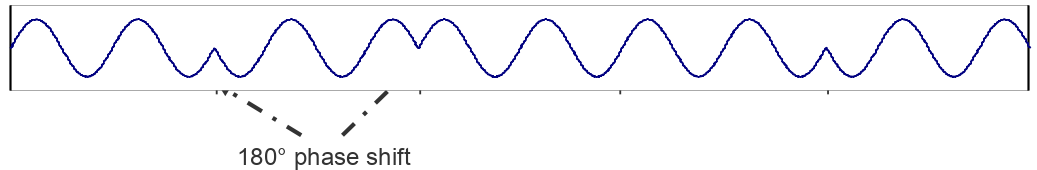
\includegraphics[width=1\textwidth]{assets/chap_2/psk_wave.png}
\end{figure}
\medskip

\noindent
\textbf{Nguyên lý hoạt động:}

\begin{itemize}
    \item Bit 1 $\rightarrow$ sóng bắt đầu ở một góc pha nhất định (như 0$^\circ$).
    \item Bit 0 $\rightarrow$ sóng bắt đầu ở góc pha khác (như 180$^\circ$).
\end{itemize}

\noindent
$\rightarrow$ Tín hiệu bị ngắt và đảo ngược trạng thái mỗi khi bit thay đổi (như hình trên, có thể thấy được ngay chỗ sóng bị đảo chiều).
\medskip

\begin{itemize}
    \item \textbf{Pros:} chống nhiễu tốt (robust against noise) $\Rightarrow$ vì nhiễu thường tác động vào biên độ, ít khi làm thay đổi pha của sóng $\Rightarrow$ ổn định hơn so với ASK; là giải pháp tổng thể tốt nhất $\rightarrow$ cân bằng giữa hiệu suất và chất lượng.
    \item \textbf{Cons:} quá trình giải điều chế phức tạp (complex demodulation process) $\Rightarrow$ receiver phải cực kì chính xác để có thể phát hiện ra sự lệch pha (dựa theo góc của sóng) $\rightarrow$ đòi hỏi phần cứng đắt tiền và phức tạp hơn so với việc chỉ cần đo độ cao (như ASK) hay đo tần số (như FSK).
\end{itemize}

\sidebox[-2cm]{Self-note:}{
$\rightarrow$ Cứ xem như PSK là 2 người chạy tiếp sức:

\begin{itemize}
    \item Bit 1 $\rightarrow$ người đầu tiên xuất phát ngay vạch xuất phát.
    \item Bit 0 $\rightarrow$ người thứ hai xuất phát ở vạch đối diện với người đầu tiên (lệch 180$^\circ$).
\end{itemize}

$\rightarrow$ Dù trời mưa có to đi chăng nữa (noise) $\Rightarrow$ vẫn biết được người đang chạy xuất phát từ đâu, do vị trí xuất phát cách rất xa nhau nên không bị nhầm.
\medskip

$\Rightarrow$ Tuy nhiên, trọng tài (receiver) phải cố nhìn mới có thể phân biệt được ai với ai (như cách máy phải chuẩn lắm mới phát hiện được, không đơn giản như ASK).
}

\subsubsection{Overview}

\noindent
\underline{Finalize:}
\medskip

\begin{center}
\begin{minipage}[c]{0.55\textwidth}
    \centering
    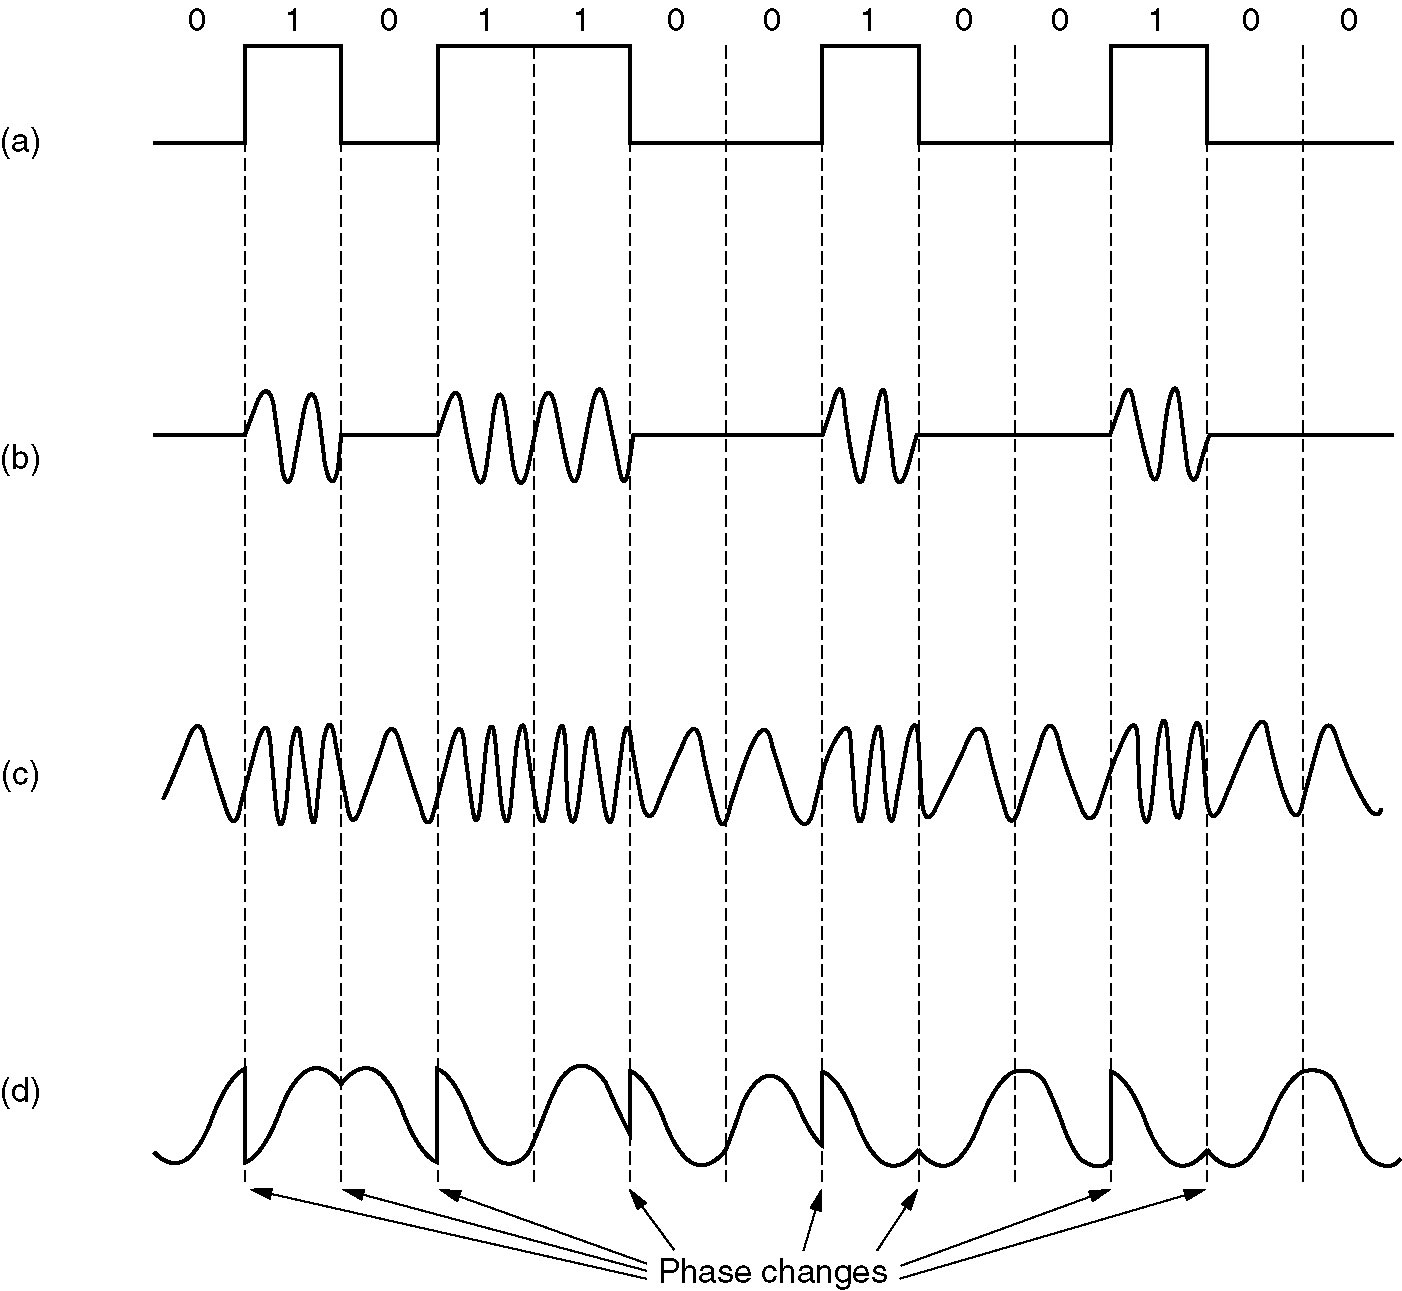
\includegraphics[width=1\textwidth]{assets/chap_2/overview.jpg}
\end{minipage}
\hfill
\begin{minipage}[c]{0.4\textwidth}
    \begin{enumerate}
        \renewcommand{\labelenumi}{\alph{enumi}.}
        \item Binary signal.
        \item Amplitude modulation.
        \item Frequency modulation.
        \item Phase modulation.
        \end{enumerate}
\end{minipage}
\end{center}

\noindent
\textbf{Binary signal (tín hiệu nhị phân):}

\begin{itemize}
    \item[$\rightarrow$] Đây là dữ liệu đầu vào (input data).
    \item[$\rightarrow$] Là các bit 0 và 1.
    \item[$\rightarrow$] Hình sóng vuông $\Rightarrow$ mức cao là 1, thấp là 0.
    \item[$\rightarrow$] Là nơi điều kiển sóng mang phải thay đổi như thế nào.
\end{itemize}
\medskip

\noindent
\textbf{Amplitude modulation (điều chế biên độ) - ASK:}

\begin{itemize}
    \item[$\rightarrow$] Binary bảo sao thì \textbf{biên độ} của sóng cũng vậy.
    \item[$\rightarrow$] Bit = 1 $\Rightarrow$ sóng dao động mạnh; bit = 0 $\Rightarrow$ sóng dao động yếu.
    \item[$\rightarrow$] Tần số và pha giữ nguyên không đổi.
\end{itemize}
\medskip

\noindent
\textbf{Frequency modulation (điều chế tần số) - FSK:}

\begin{itemize}
    \item[$\rightarrow$] Binary bảo sao thì \textbf{tần số} của sóng cũng vậy.
    \item[$\rightarrow$] Bit = 1 $\Rightarrow$ sóng bị ép lại, dao động nhanh (tần số cao); bit = 0 $\Rightarrow$ sóng giãn ra, dao động chậm (tần số thấp).
    \item[$\rightarrow$] Biên độ và pha giữ nguyên không đổi.
\end{itemize}
\medskip

\clearpage

\noindent
\textbf{Phase modulation (điều chế pha) - PSK:}

\begin{itemize}
    \item[$\rightarrow$] Binary thay đổi (từ 0 $\rightarrow$ 1 hoặc 1 $\rightarrow$ 0) thì sóng phải \textbf{đảo chiều} (đổi pha).
    \item[$\rightarrow$] Mỗi khi bit thay đổi $\rightarrow$ sóng bị gãy và đi xuống (hoặc ngược lại) $\Rightarrow$ tạo sự lệch pha (nhằm để phân biệt giữa 2 bit khác nhau).
    \item[$\rightarrow$] Biên độ và tần số giữ nguyên không đổi (sóng cao bằng nhau và nhanh như nhau).
\end{itemize}
\medskip

\section{Transmission Media}

\subsection{Classification of Transmission Media}

\noindent
Mô hình tổng thể:

\begin{figure}[ht]
    \centering
    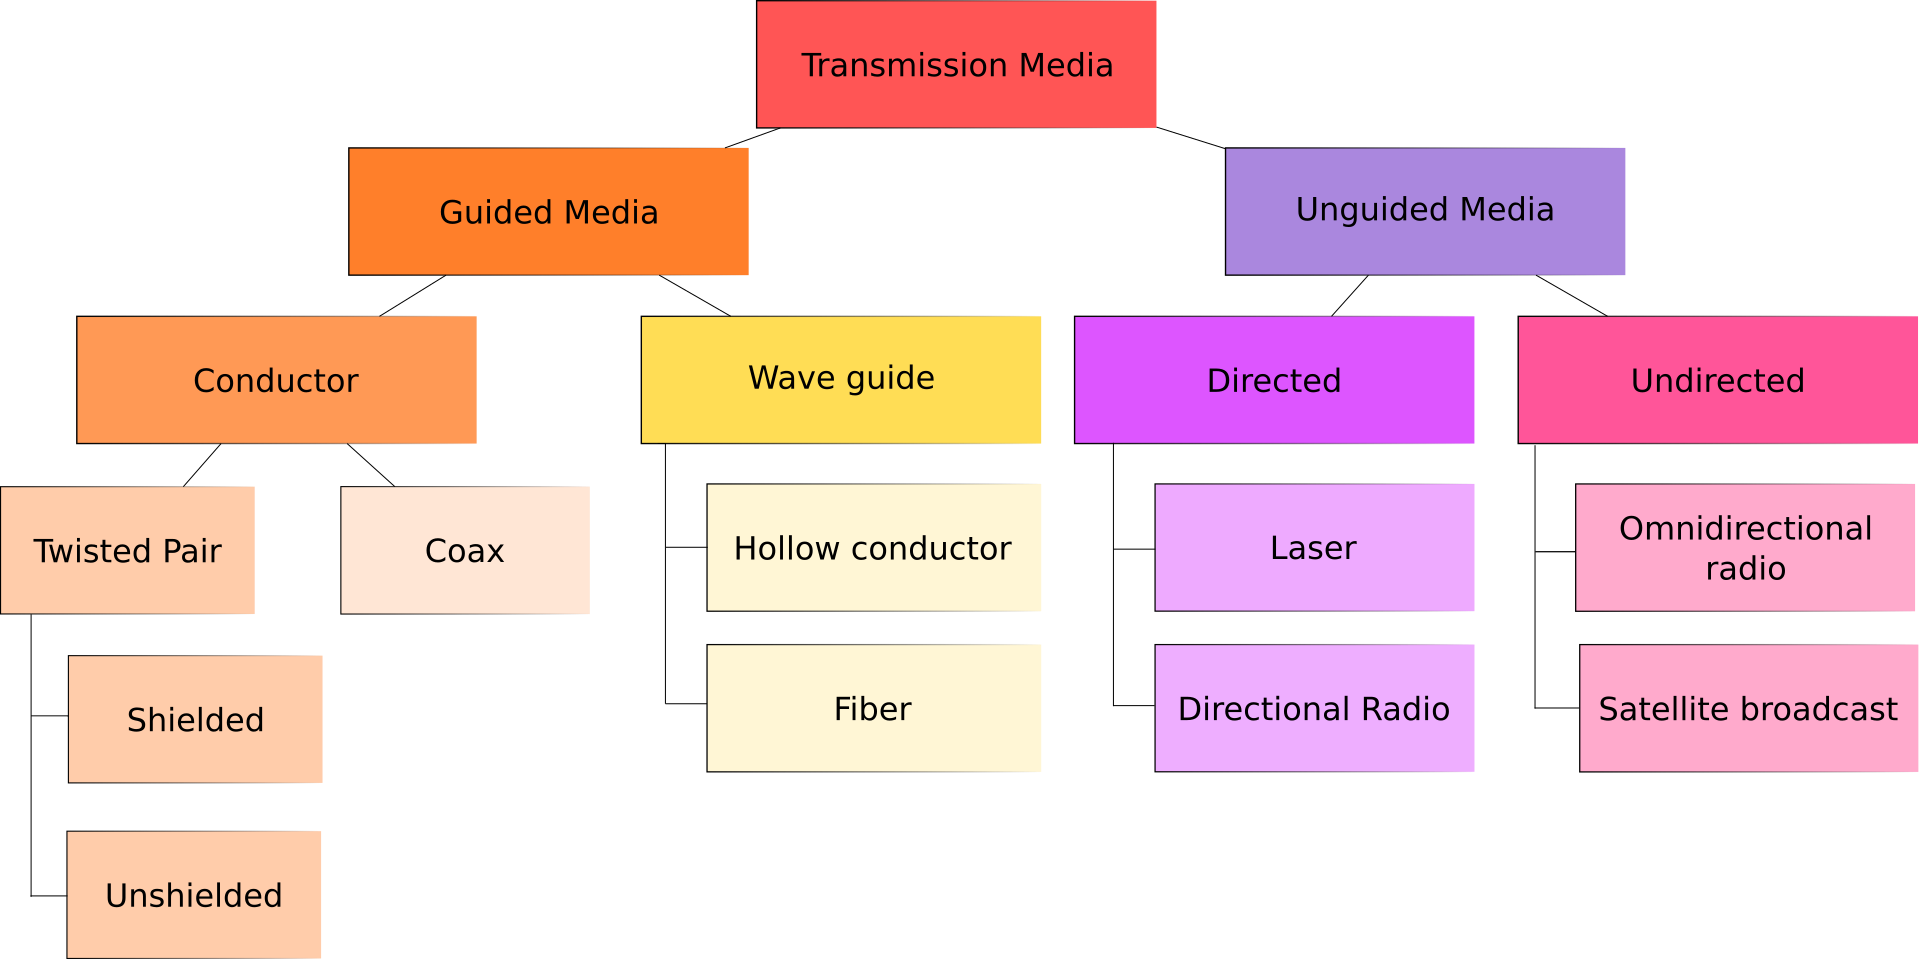
\includegraphics[width=0.78\textwidth]{assets/chap_2/class_trans_med.png}
\end{figure}
\medspace

$\rightarrow$ Chia làm 2 loại chính: \textbf{guided media} (phương tiện hữu tuyến) và \textbf{unguided media} (phương tiện vô tuyến).
\medskip

\subsection{Guided Transmission Media}

\noindent
Guided transmission media (phương tiện truyền dẫn có hướng) $\rightarrow$ tín hiệu được dẫn đường cụ thể bên trong một vật thể vật lý (như dây dẫn chẳng hạn).

$\Rightarrow$ Tín hiệu không truyền bên ngoài.
\medskip

\noindent
Được chia làm \textbf{2 loại}:

\begin{itemize}
    \item Conductor (dây dẫn) $\rightarrow$ dùng dòng điện để truyền tín hiệu.
    \item Wave guide (dẫn sóng) $\rightarrow$ dùng sóng ánh sáng (light waves) để truyền tín hiệu.
\end{itemize}

\subsubsection{Coaxial Cables (Coax Cables)}

\noindent
Coaxial cable (cáp đồng trục) $\rightarrow$ là loại dây dẫn hữu tuyến phổ biến (dùng cho truyền hình cáp, mạng thế hệ cũ, ...).
\medskip

\begin{figure}[H]
    \centering
    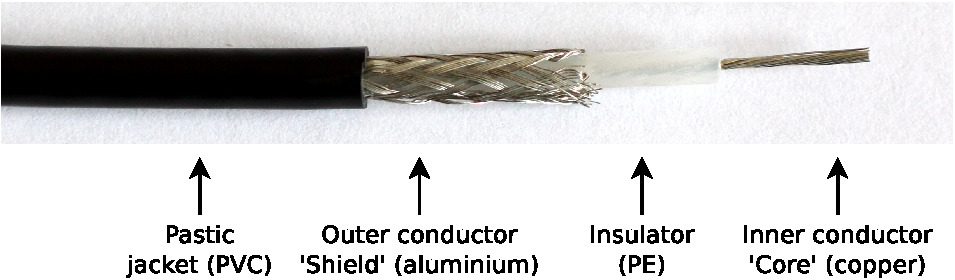
\includegraphics[width=0.9\textwidth]{assets/chap_2/coaxial.jpg}
\end{figure}
\medspace

\noindent
$\rightarrow$ Một loại cáp đồng trục dùng để mang tín hiệu bipolar.
\medskip

\noindent
\textbf{Cấu tạo:}

\begin{itemize}
    \item \textbf{Inner conductor} (dây dẫn bên trong) $\rightarrow$ thường làm bằng đồng $\Rightarrow$ có nhiệm vụ mang tín hiệu điện (carries electrical signal) $\rightarrow$ đây là nơi dữ liệu chạy qua.
    \item \textbf{Insulation} (lớp cách điện) $\rightarrow$ làm bằng nhựa PE $\Rightarrow$ ngăn cách, không cho lõi chạm vào lớp vỏ lưới bên ngoài nhằm tránh chập mạch.
    \item \textbf{Outer conductor/shield} (lớp vỏ dẫn điện) $\rightarrow$ được làm bằng nhôm hoặc lưới kim loại $\Rightarrow$ có nhiệm vụ giữ mức điện thế đất (ground potential); bao bọc xung quanh lõi hòng ngăn chặn nhiễu điện từ (noise) từ bên ngoài xâm nhập vào lõi.
    \item \textbf{Plastic jacket} (lớp vỏ nhựa) $\rightarrow$ bảo vệ vật lý cho sợi cáp (chống nước, trầy xước các kiểu).
\end{itemize}
\medskip

\sidebox[-4cm]{Self-note:}{Tín hiệu dạng bipolar là tín hiệu điện có 3 mức điện áp: dương (+V), âm (-V) và không (0V) $\rightarrow$ thường dùng nhiều trong viễn thông và một số hệ thống truyền dữ liệu.}

\subsubsection{Twisted Pair Cables}

\noindent
Twisted pair cable (cáp xoắn đôi) $\rightarrow$ là loại dây dẫn hữu tuyến phổ biến nhất, rẻ nhất, thường thấy dùng trong mạng LAN (Ethernet) và điện thoại bàn.
\medskip

\noindent
$\rightarrow$ Dây của cáp xoắn đôi được xoắn cặp (pairwise twisted) với nhau.
\medskip

\noindent
\textbf{Cấu tạo cơ bản:} gồm 2 dây dẫn đồng được bọc cách điện.
\medskip

\noindent
\textbf{Nguyên tắc "twist":} 2 sợ dây đồng được xoắn lại như buộc tóc đuôi sam $\rightarrow$ để chống nhiễu từ (EMI - Electromagnetic Interference) và crosstalk (xuyên âm) giữa các cặp dây bên trong.

$\Rightarrow$ Twisted pairs are better protected against alternating magnetic fields and electrostatic interference from the outside than parallel signal wires.
\medskip

\noindent
\textbf{Công dụng của việc xoắn:}

\begin{itemize}
    \item Chống nhiễu (EMI) từ tác động bên ngoài $\rightarrow$ do xoắn, sóng nhiễu sẽ tác động lên mỗi sợi dây trong cặp ngược chiều nhau $\Rightarrow$ khi receiver đọc tín hiệu (bằng cách lấy hiệu giữa 2 sợi dây) thì nhiễu sẽ tự động triệt tiêu.
    \item Chống xuyên âm (crosstalk) từ trong $\rightarrow$ mỗi cặp dây có tốc độ xoắn khác nhau $\Rightarrow$ giảm thiểu tối đa lượng nhiễu bị truyền từ cặp này sang cặp khác.
\end{itemize}

\begin{figure}[H]
    \centering
    \begin{minipage}{0.6\textwidth}
        \centering
        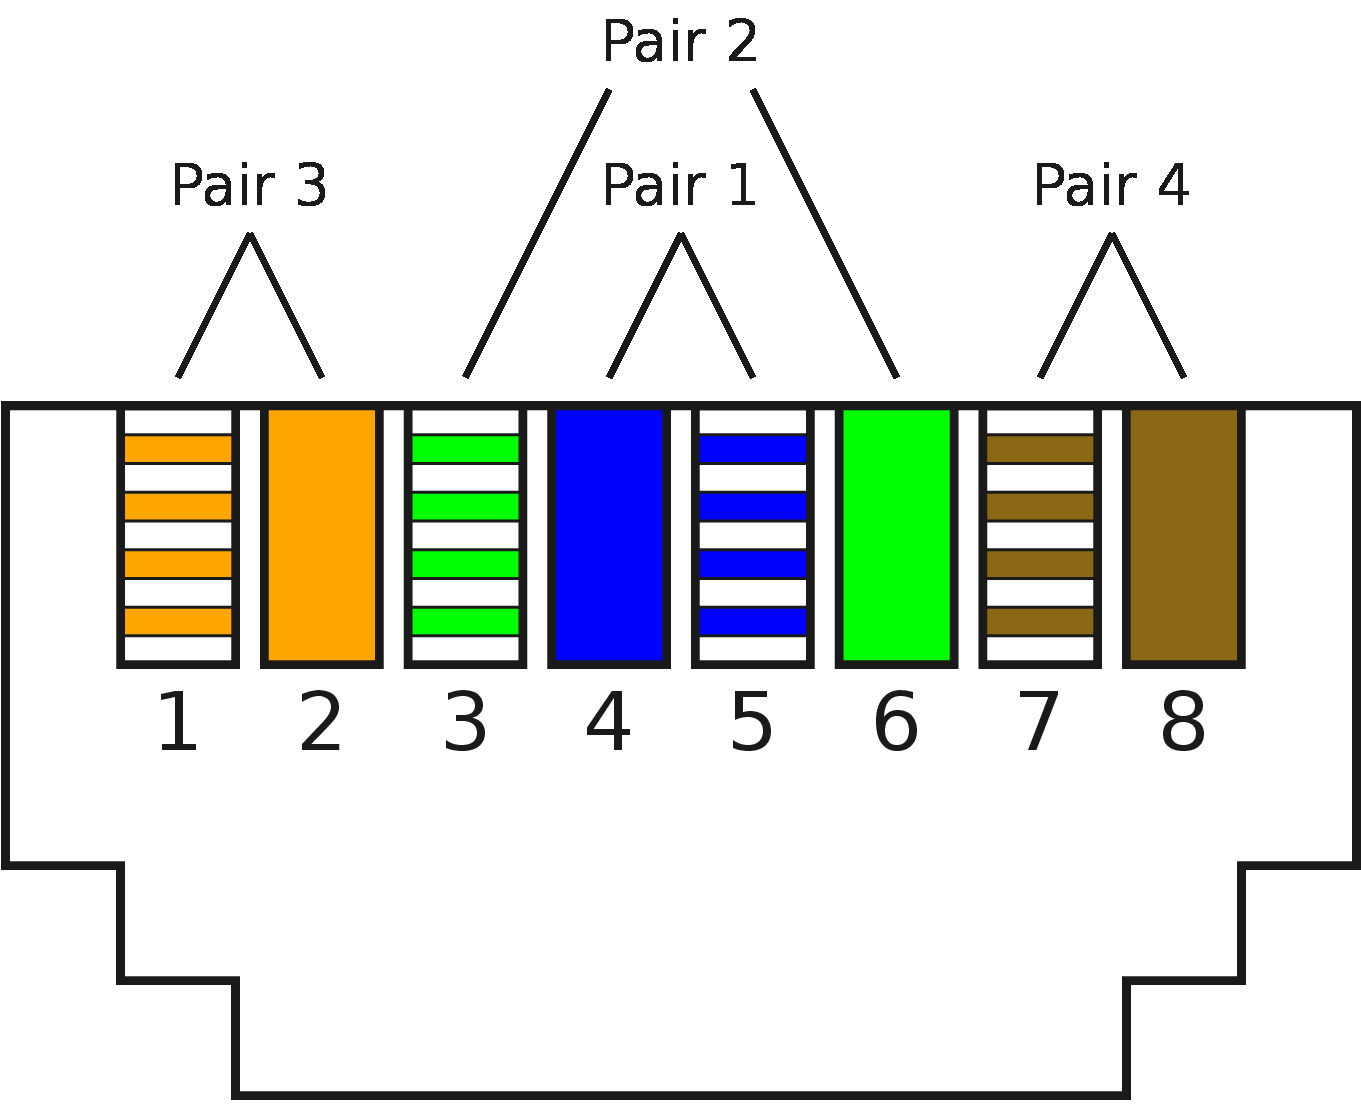
\includegraphics[width=0.6\textwidth]{assets/chap_2/tp_dia.jpg}
    \end{minipage}
    \hfill
    \begin{minipage}{0.3\textwidth}
        \centering
        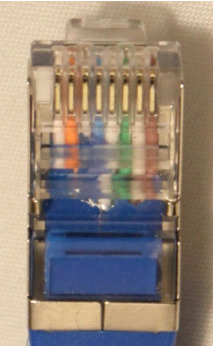
\includegraphics[width=0.65\textwidth]{assets/chap_2/tp_cable_1.jpg}
    \end{minipage}
\end{figure}
\medskip

\noindent
$\rightarrow$ Tất cả các chuẩn Ethernet dùng cáp xoắn đôi đều sử dụng đầu nối 8P8C, thường gọi là RJ45 (Registered Jack).
\medskip

\sidebox[-6.3cm]{Self-note:}{
\begin{itemize}
    \item Xuyên âm $\rightarrow$ là sự nhiễu loạn lẫn nhau giữa các dây dẫn chạy song song $\Rightarrow$ khi dòng điện chạy trong dây dẫn thứ nhất, nó sẽ tạo ra từ trường xung quanh nó $\rightarrow$ từ trường này gây hiện tượng cảm ứng sang dây kế bên mà nó nằm song song, tạo ra một dòng điện không mong muốn trên dây kia.
    \item EMI $\rightarrow$ là nhiễu do các nguồn bên ngoài phát ra, tác động vào sợi cáp (như sấm sét, tia lửa điện, vi sóng, thiết bị Bluetooth, ...).
\end{itemize}
}

\subsubsection{Shielding of different Twisted Pair Cables}

\noindent
$\rightarrow$ Cáp xoắn đôi thường được trang bị thêm lớp vỏ kim loại (medal shield) $\Rightarrow$ ngăn chặn nhiễu điện từ (EMI) từ bên ngoài.
\medskip

\noindent
$\rightarrow$ Các cặp dây hoặc toàn bộ sợi cáp có thể được bọc thêm lớp chống nhiễu (bằng lưới kim loại (braided shield) hoặc lá kim loại (foil shield)).

$\Rightarrow$ Lớp chống nhiễu chỉ hiệu quả khi hai đầu cáp được nối đất tại cùng một điện thế (ground potential).
\medskip

\noindent
\underline{Self-note:} hai đầu cáp phải nối đất cùng một hiệu điện thế $\rightarrow$ do lớp chống nhiễu chỉ hoạt động đúng khi không có dòng điện chạy qua (đúng nghĩa cái từ "chống nhiễu").

$\rightarrow$ Theo định luật Ohm, nếu có hiệu điện thế chênh lệch thì sẽ có dòng điện chạy qua.
\medskip

\noindent
\textbf{UTP:} Unshielded Twisted Pair (cáp xoắn không vỏ bọc) $\rightarrow$ không có lớp vỏ kim loại bảo vệ bên ngoài.
\medskip

\begin{center}
\begin{minipage}[c]{0.35\textwidth}
    \centering
    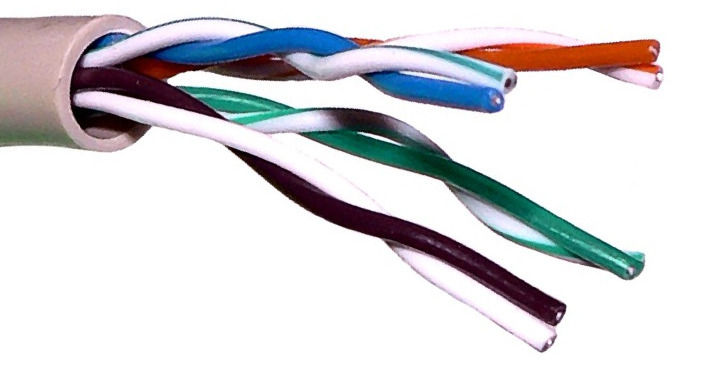
\includegraphics[width=0.8\textwidth]{assets/chap_2/utp.jpg}
\end{minipage}
\hfill
\begin{minipage}[c]{0.6\textwidth}
    \begin{itemize}
        \item[$\rightarrow$] Chỉ có dây đồng xoắn và lớp vỏ nhựa PVC.
        \item[$\Rightarrow$] Rẻ và phổ biến nhất, nhưng chống nhiễu kém (chỉ dựa theo nguyên lý xoắn dây để chống).
    \end{itemize}
\end{minipage}
\end{center}
\medskip

\noindent
\textbf{FTP / F-UTP:} Foiled Twisted Pair (cáp xoắn đôi có lá bọc) $\rightarrow$ có lớp lá kim loại bọc bên ngoài từng cặp dây.
\medskip

\begin{center}
\begin{minipage}[c]{0.35\textwidth}
    \centering
    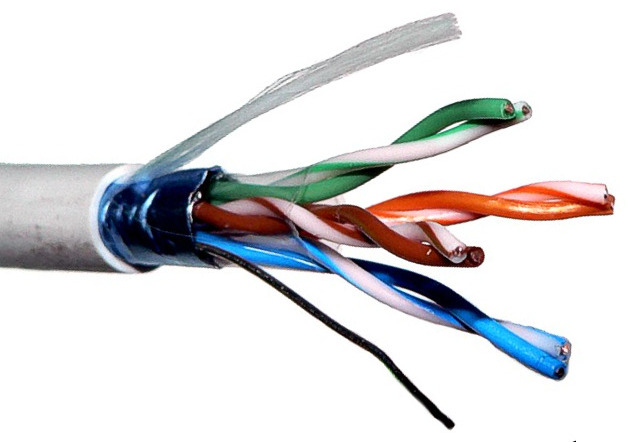
\includegraphics[width=0.8\textwidth]{assets/chap_2/ftp.jpg}
\end{minipage}
\hfill
\begin{minipage}[c]{0.6\textwidth}
    \begin{itemize}
        \item[$\rightarrow$] Các cặp dây được bao bọc bởi một lớp kim loại mỏng bao quanh toàn bộ bó dây (twisted pairs).
        \item[$\Rightarrow$] Chống nhiễu tốt hơn UTP một xíu.
    \end{itemize}
\end{minipage}
\end{center}
\medskip

\clearpage

\noindent
\textbf{SFTP:} Shielded Foiled Twisted Pair (cáp xoắn đôi có lá bọc và vỏ bọc) $\rightarrow$ có lớp lá kim loại bọc bên ngoài từng cặp dây, đồng thời có lớp lưới kim loại bọc bên ngoài toàn bộ bó dây.
\medskip

\begin{center}
\begin{minipage}[c]{0.35\textwidth}
    \centering
    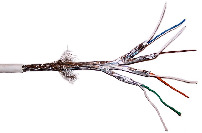
\includegraphics[width=0.8\textwidth]{assets/chap_2/sftp.jpg}
\end{minipage}
\hfill
\begin{minipage}[c]{0.5\textwidth}
    \centering
    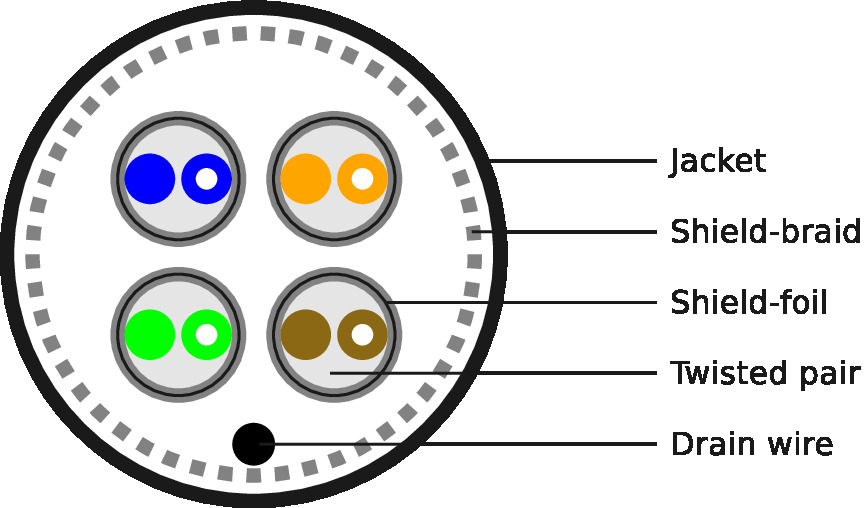
\includegraphics[width=0.8\textwidth]{assets/chap_2/sftp-struct.jpg}
\end{minipage}
\end{center}
\medskip

\begin{itemize}
    \item Shield-foil $\rightarrow$ từng cặp dây hoặc bó dây được bao bọc lá nhôm.
    \item Shield-braid $\rightarrow$ ngoài cùng có thêm một một lớp lưới kim loại (braided).
    \item Drain wire $\rightarrow$ dây nối đất (ground wire) để dòng điện nhiễu xuống đất.
    \item[$\Rightarrow$] Chống nhiễu cực tốt, cáp rất to, chi phí đắt.
\end{itemize}
\medskip

\subsubsection{Categories of Twisted Pair Cables}

\noindent
\textbf{Nguyên tắc:}
\medskip

\noindent
Hiệu suất của toàn bộ kết nối được quyết định từ category thấp nhất $\rightarrow$ ví dụ như dùng Cat 7 (xịn nhất) mà đi cắm vào một cái ổ siêu lỗi thời (như Cat 5 chẳng hạn) thì tốc độ nó sẽ ở mức của Cat 5 chứ không phải ngang mức cái dây.
\medskip

\begin{itemize}
    \item Cat 1/2/3/4 $\rightarrow$ đã lỗi thời. Nay chỉ dùng cho điện thoại bàn.
    \item Cat 5/5e $\rightarrow$ phổ biến trong các mạng LAN ngày nay; có tốc độ ổn cho các nhu cầu bình thường (100Mbps - 1Gbps).
    \item Cat 6/6A $\rightarrow$ có tốc độ cao, hỗ trợ lên đến 10Gbps ở khoảng cách 100m; dùng cho mạng đòi hỏi tốc độ nhanh.
    \item Cat 7/7A $\rightarrow$ thật ra chả có lợi gì hơn so với Cat 6A.
    \item Cat 8 $\rightarrow$ được thiết kế cho các data center; hỗ trợ với tốc độ cực cao nhưng chỉ với khoảng cách ngắn ($\approx$30m).
\end{itemize}

\noindent
\textbf{Câu hỏi:} Tại sao Cat càng lớn càng xịn hơn, nhanh hơn?

$\Rightarrow$ Number of twists (số vòng xoắn) per wire length (cm) and thickness of the jacket (lớp vỏ bọc bên ngoài).

\begin{itemize}
    \item Càng xoắn nhiều vòng $\Rightarrow$ càng ít nhiễu (more twists $\Rightarrow$ less interference).
    \item Lớp vỏ bọc càng dày $\Rightarrow$ càng chống nhiễu tốt (thickness of the cladding (lớp bao phủ) $\Rightarrow$ less crosstalk).
\end{itemize}
\medskip

\noindent
$\rightarrow$ Cat 5/5e có 1-2 vòng xoắn trên mỗi cm. Cat 6 có 2 vòng xoắn trở lên trên mỗi cm.
\medskip

\noindent
$\rightarrow$ Crosstalk là hiện tượng tín hiệu bị nhiễu lẫn nhau giữa các đường dây song song.
\medskip

\subsubsection{Fiber-optic Cables}

\noindent
Fiber-optic cable (cáp quang) $\rightarrow$ là loại dây dẫn hữu tuyến dùng sóng ánh sáng để truyền tín hiệu thay vì dây lõi đồng.
\medskip

\begin{center}
\begin{minipage}[c]{0.45\textwidth}
    \centering
    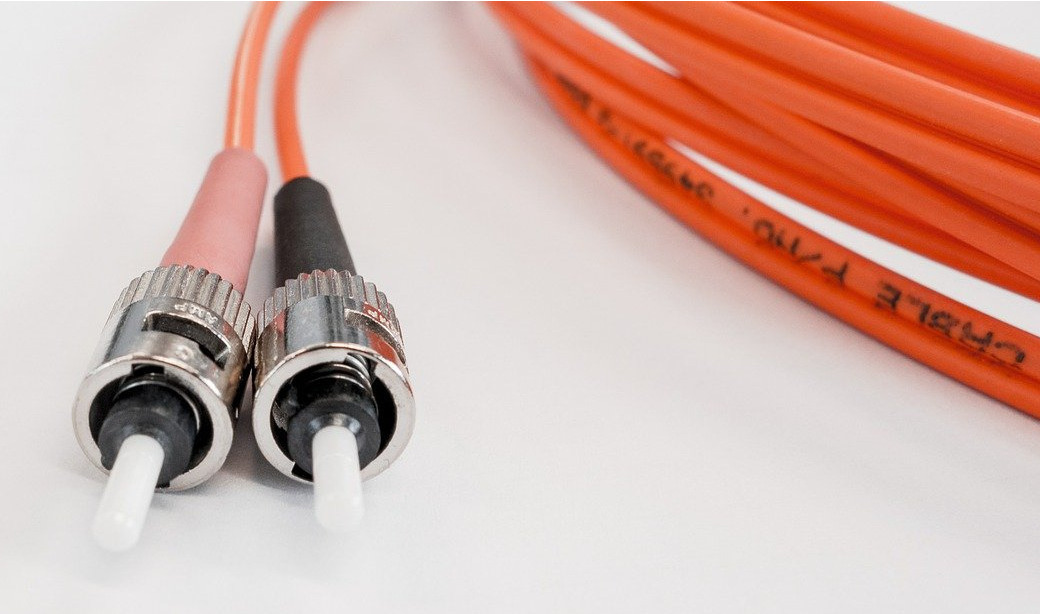
\includegraphics[width=1\textwidth]{assets/chap_2/fiber_1.jpg}
\end{minipage}
\hfill
\begin{minipage}[c]{0.45\textwidth}
    \centering
    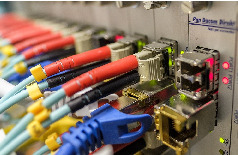
\includegraphics[width=0.9\textwidth]{assets/chap_2/fiber_2.jpg}
\end{minipage}
\end{center}
\medskip

\noindent
\textbf{Nguyên lý hoạt động:}

\begin{itemize}
    \item Light source (nguồn sáng) $\rightarrow$ sử dụng đèn LED hoặc laser LED để bắn tín hiệu.
    \item Use wavelengths (dùng bước sóng) $\rightarrow$ sử dụng các bước sóng 850, 1300, hoặc 1550 nm.
    \item Môi trường truyền $\rightarrow$ ánh sáng chạy trong sợi thủy tinh với tốc độ gần 200,000 km/s.
\end{itemize}

\noindent
\textbf{So sánh với coaxial (cáp đồng trục) và twisted pair (cáp xoắn đôi):}
\medskip

\noindent
\textbf{Pros:}

\begin{itemize}
    \item High data rates and large distances $\rightarrow$ tốc độ cực cao và truyền được rất xa (hàng chục km không cần khuếch đại).
    \item No electromagnetic emission $\rightarrow$ không phát sóng điện từ ra ngoài $\Rightarrow$ rất khó bị leak (bảo mật cao).
    \item Insensitive against electromagnetic interference (miễn nhiễm với EMI) $\rightarrow$ do nó là ánh sáng nên không sợ sấm sét hay điện lưới gây nhiễu.
\end{itemize}
\medskip

\textbf{Cons:}

\begin{itemize}
    \item Higher cost $\rightarrow$ chi phí cáp và thiết bị (như các module quang/LED) đắt đỏ hơn so với dây đồng.
    \item Infrastructure $\rightarrow$ không thể tận dụng được hạ tầng cũ (như dây đồng) $\Rightarrow$ phải xây mới hoàn toàn.
\end{itemize}

\noindent
$\rightarrow$ Chỉ dùng khi cáp đồng không thể cung cấp đủ bandwidth hoặc khoảng cách quá xa.
\medskip

\subsection{Unguided Transmission Media}

\noindent
Unguided transmission media (phương tiện truyền dẫn vô tuyến) $\rightarrow$ tín hiệu không chạy trong một vật thể vật lý (như dây cáp) mà truyền tự do trong không gian (như không khí, chân không).

$\Rightarrow$ Tín hiệu truyền tự do ra bên ngoài.

\begin{itemize}
    \item Directed (có hướng) $\rightarrow$ tín hiệu được tập trung thành một chùm tia hẹp (beam) bắn thẳng từ máy phát đến máy thu $\Rightarrow$ yêu cầu hai thiết bị phải thấy nhau (line-of-sight), không có vật cản ở giữa; ví dụ như điều khiển TV.
    \item Undirected (vô hướng/đa hướng) $\rightarrow$ sóng được phát mọi hướng $\Rightarrow$ máy thu có thể ở bất kì nơi nào trong vùng phủ sóng là được; ví dụ: truyền hình vệ tinh (satellite TV).
\end{itemize}
\medskip

\subsubsection{Wireless Communication}

\begin{figure}[htbp]
    \centering
    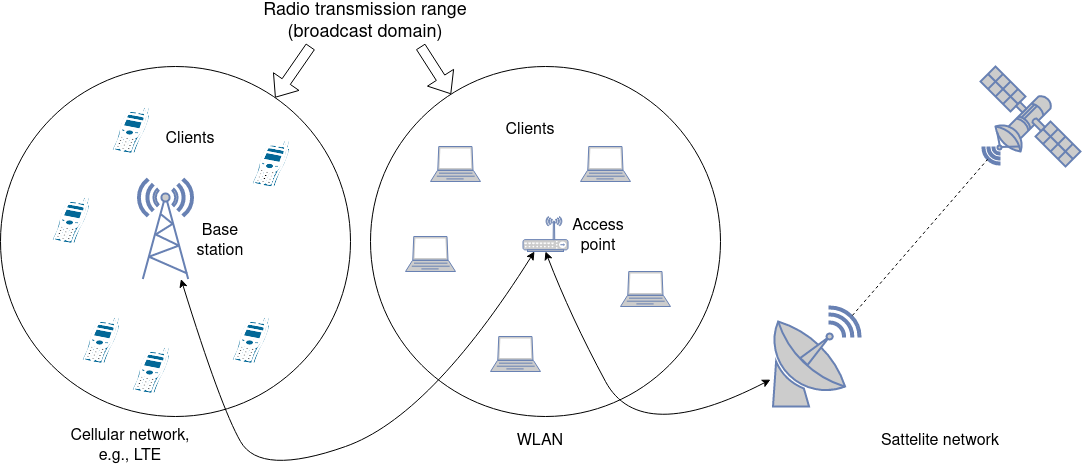
\includegraphics[width=0.75\textwidth]{assets/chap_2/wireless.png}
\end{figure}

\noindent
\textbf{Đặc điểm kĩ thuật:}

\begin{itemize}
    \item Medium is an electromagnetic wave $\rightarrow$ môi trường truyền là sóng điện từ.
    \item Data is modulated $\rightarrow$ dữ liệu được điều chế lên sóng mang.
    \item Range $\rightarrow$ phụ thuộc vào công suất phát (signal power) và môi trường (environment).
    \item Can be directed or undirected $\rightarrow$ có thể định hướng (như sóng micro) hoặc không định hướng (như sóng radio).
\end{itemize}
\medskip

\noindent
\textbf{Shared medium} (môi trường truyền dẫn chung) $\rightarrow$ các tần số không thể sử dụng tùy ý muốn (cannot be used arbitrarily) mà phải được phân bổ (must be allocated).
\medskip

\subsubsection{Challenges of Wireless Networks}

\noindent
\textbf{Fading over distance} (suy giảm tín hiệu theo khoảng cách)
\medskip

\noindent
$\rightarrow$ Sóng điện từ suy giảm bị yếu dần (gradually weaken) khi truyền trong không gian hoặc gặp vật cản vật lý (chẳng hạn như tường).

$\Rightarrow$ Càng đi xa Wifi hay vào chỗ khuất $\rightarrow$ sóng càng yếu $\Rightarrow$ mạng yếu đi hoặc mất kết nối.
\medskip

\begin{figure}[H]
    \centering
    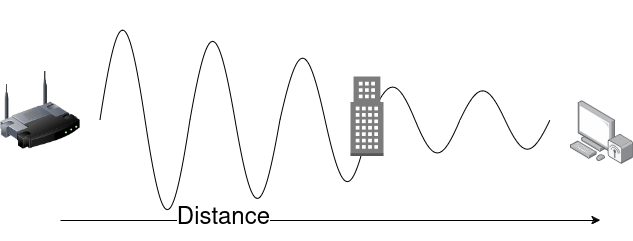
\includegraphics[width=0.55\textwidth]{assets/chap_2/fading.png}
\end{figure}
\medskip

\clearpage

\noindent
\textbf{Exposed terminal problem} (vấn đề "trạm lộ thiên")
\medskip

\begin{figure}[H]
    \centering
    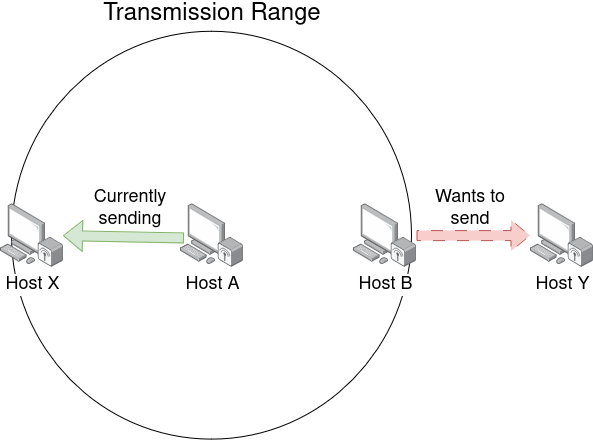
\includegraphics[width=0.55\textwidth]{assets/chap_2/exposed.png}
\end{figure}
\medskip

\noindent
$\rightarrow$ Máy B (theo hình trên) muốn gửi dữ liệu cho máy Y; tuy nhiên thì máy B đang nằm trong vùng phủ sóng của máy A, và máy A đang bận gửi tin cho máy X.
\medskip

\noindent
A node is prevented from sending packets to other nodes because of being within transmission range of a neighboring transmitter.

$\Rightarrow$ Máy B bị chặn không cho gửi dữ liệu đến máy Y (theo quy tắc CSMA sẽ được mention sau: trước khi muốn truyền dữ liệu thì phải xem môi trường có máy nào đang truyền không) $\rightarrow$ lãng phí băng thông, giảm hiệu suất mạng.
\medskip

\noindent
\textbf{Hidden terminal problem} (vấn đề "trạm ẩn"; invisible or hidden terminal devices)
\medskip

\begin{figure}[H]
    \centering
    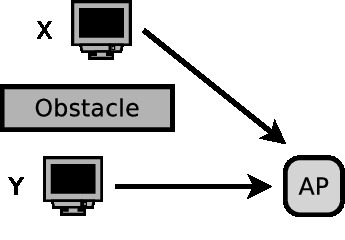
\includegraphics[width=0.45\textwidth]{assets/chap_2/hidden.jpg}
\end{figure}
\medskip

\noindent
$\rightarrow$ 2 thiết bị (như hình trên) nằm ở hai vị trí đối diện của một bức tường (đóng vai trò là vật cản). Cả 2 thiết bị không nhìn thấy nhau, muốn nói chuyện với cục AP (Access Point) ở giữa.

$\Rightarrow$ X nghĩ không có dữ liệu nào đang truyền cho cục AP, và Y cũng nghĩ như thế $\rightarrow$ cả 2 tín hiệu cùng truyền lên AP $\Rightarrow$ bị xung đột (collision), AP không nghe được cái nào cả.
\medskip

\clearpage

\noindent
\textbf{Multipath propagation} (đa đường truyền)
\medskip

\begin{figure}[H]
    \centering
    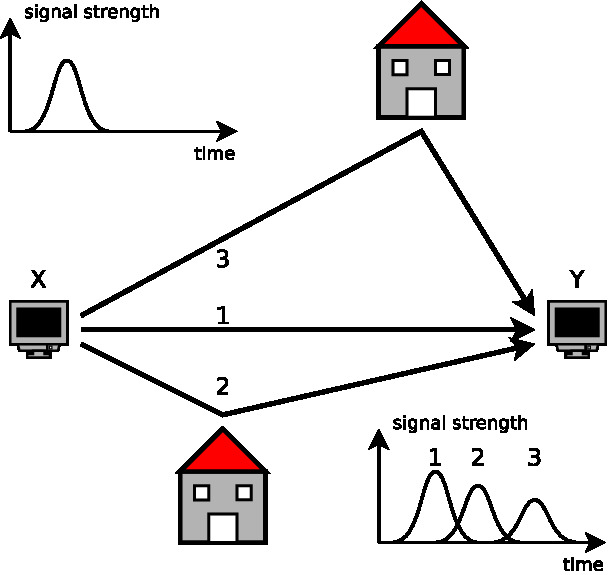
\includegraphics[width=0.45\textwidth]{assets/chap_2/multipath.jpg}
\end{figure}
\medskip

\noindent
\textbf{Giải thích:} (theo hình trên)

\begin{itemize}
    \item Một phần sóng đi thẳng đến receiver (đường số 1).
    \item Các phần sóng khác bị phản xạ từ tường (đường số 2 và 3) rồi mới đến receiver.
    \item[$\rightarrow$] Do các quãng đường có độ dài khác nhau $\Rightarrow$ chúng sẽ tới receiver vào những thời điểm khác nhau.
\end{itemize}
\medskip

\noindent
$\rightarrow$ Sóng điện từ bị phản xạ (reflected) $\rightarrow$ các đường truyền có độ dài khác nhau từ nơi gửi đến nơi nhận $\Rightarrow$ tín hiệu khó có thể giải mã do phản xạ làm ảnh hưởng đến các tín hiệu tiếp theo.

$\rightarrow$ Nếu các objects di chuyển giữa sender và receiver $\Rightarrow$ đường truyền có thể bị thay đổi.
\medskip

\noindent
\textbf{External interference} (nhiễu từ bên ngoài)
\medskip

\noindent
\textbf{$\rightarrow$ Vấn đề:} môi trường truyền phi vật lý là môi trường truyền dẫn chung (shared medium).

$\Rightarrow$ Các tín hiệu phải cạnh tranh nhau để sử dụng tần số (frequency), hoặc bị nhiễu từ các thiết bị điện tử khác.
\medskip

\noindent
\textbf{Ví dụ:}

\begin{itemize}
    \item WLAN và Bluetooth cùng sử dụng chung tần số (same spectrum); cùng dùng chung 2.4 GHz $\Rightarrow$ gây cạnh tranh đường truyền.
    \item Electromagnetic noise từ các thiết bị như lò vi sóng, hay motor, khi hoạt động cũng phát ra sóng gây nhiễu.
\end{itemize}
\medskip
\noindent

\subsection{The Last Mile}

$\rightarrow$ Là đoạn kết nối cuối cùng từ trạm cung cấp (ISP - Internet Service Provider) đến người dùng (customer premises).
\medskip

\subsubsection{Bridging the Last Mile}

\noindent
\textbf{$\rightarrow$ Vấn đề:} làm thế nào để kết nối hàng triệu người dùng vào mạng Internet với chi phí rẻ nhất (cost-efficient)?
\medskip

\clearpage

\noindent
\underline{Common solutions:}

\begin{itemize}
    \item \textbf{DSL (Digital Subscriber Line)} $\rightarrow$ tận dụng đường dây điện thoại (access through phone lines).
    \item \textbf{Cable} $\rightarrow$ tận dụng tín hiệu truyền hình cáp (access through TV broadcast system).
    \item \textbf{3G/4G} $\rightarrow$ tận dụng các trạm phát sóng di động (access through deployed cellular networks).
\end{itemize}
\medskip

\noindent
\underline{Other solutions:}

\begin{itemize}
    \item \textbf{Powerline} $\rightarrow$ Internet truyền qua đường dây điện trong nhà (AC infrastructure).
    \item \textbf{Satellite} $\rightarrow$ dùng vệ tinh (chẳng hạn như Starlink của Elon Musk) $\Rightarrow$ có thể phủ sóng vùng sâu vùng xa.
    \item \textbf{Wireless} $\rightarrow$ như WiMAX, directed WIFI.
    \item \textbf{Fiber (cáp quang)} $\rightarrow$ có tốc độ cao nhất, nhưng rất tốn kém do phải xây đường đi dây mới hoàn toàn (rerquires infrastructure expansion).
\end{itemize}

\subsubsection{History: The Classical Modem}

\noindent
Modem (modulator-demodulator) $\rightarrow$  chuyển đổi dữ liệu số (digital data, bit 0, 1) từ máy tính sáng tín hiệu tương tự (analog) để truyền đi và ngược lại.
\medskip

\noindent
\textbf{$\rightarrow$ Nguyên lý hoạt động:} sử dụng đường dây điện thoại cố định (POTS - Plain Old Telephone Service) $\rightarrow$ modem truyền dữ liệu giống như cách truyền tín hiệu radio bình thường (normal audio signals) $\Rightarrow$ biến các bit dữ liệu thành các âm thanh.

$\Rightarrow$ Modem chịu trách nhiệm xử lý thông tin tín hiệu (takes care of the signaling information).
\medskip

\noindent
\textbf{Đặc điểm kĩ thuật:}

\begin{itemize}
    \item High error rate (tỉ lệ lỗi cao) $\rightarrow$ do đường dây điện thoại vốn chỉ thiết kế cho giọng nói $\Rightarrow$ rất dễ bị nhiễu và dẫn đến làm sai dữ liệu.
    \item Speed (tốc độ) $\rightarrow$ rất chậm, tốc độ tối đa chỉ đạt cỡ 56 kbps.
\end{itemize}
\medskip

\begin{figure}[htbp]
    \centering
    
\includegraphics[width=0.8\textwidth]{assets/chap_2/class_modem.png}
\end{figure}
\medskip

\noindent
$\rightarrow$ Modem cổ điển tựa như việc đọc chính tả cho phía bên kia chép vậy.
\medskip

\subsubsection{Digital Subscriber Line (DSL)}

\noindent
DSL (đường dây thuê bao số) $\rightarrow$ là công nghệ tiên tiến của mạng điện thoại cố định (POTS) để truyền tốc độ cao.

$\rightarrow$ Tận dụng được hạ tầng cũ $\Rightarrow$ vẫn dùng sợi cáp đồng của điện thoại bàn.
\medskip

\begin{center}
\begin{minipage}[c]{0.55\textwidth}
    \noindent
    \textbf{Điểm khác:} (so với modem cổ điển)

    \begin{itemize}
        \item Modem cũ chỉ dùng một dãy tần số âm thanh rất hẹp, chỉ để vừa đủ nghe tiếng nói.
        \item DSL khai thác toàn bộ phổ tần (whole spectrum) của sợi cáp đồng để nhồi nhét dữ liệu vào.
    \end{itemize}
\end{minipage}
\hfill
\begin{minipage}[c]{0.35\textwidth}
    \centering
    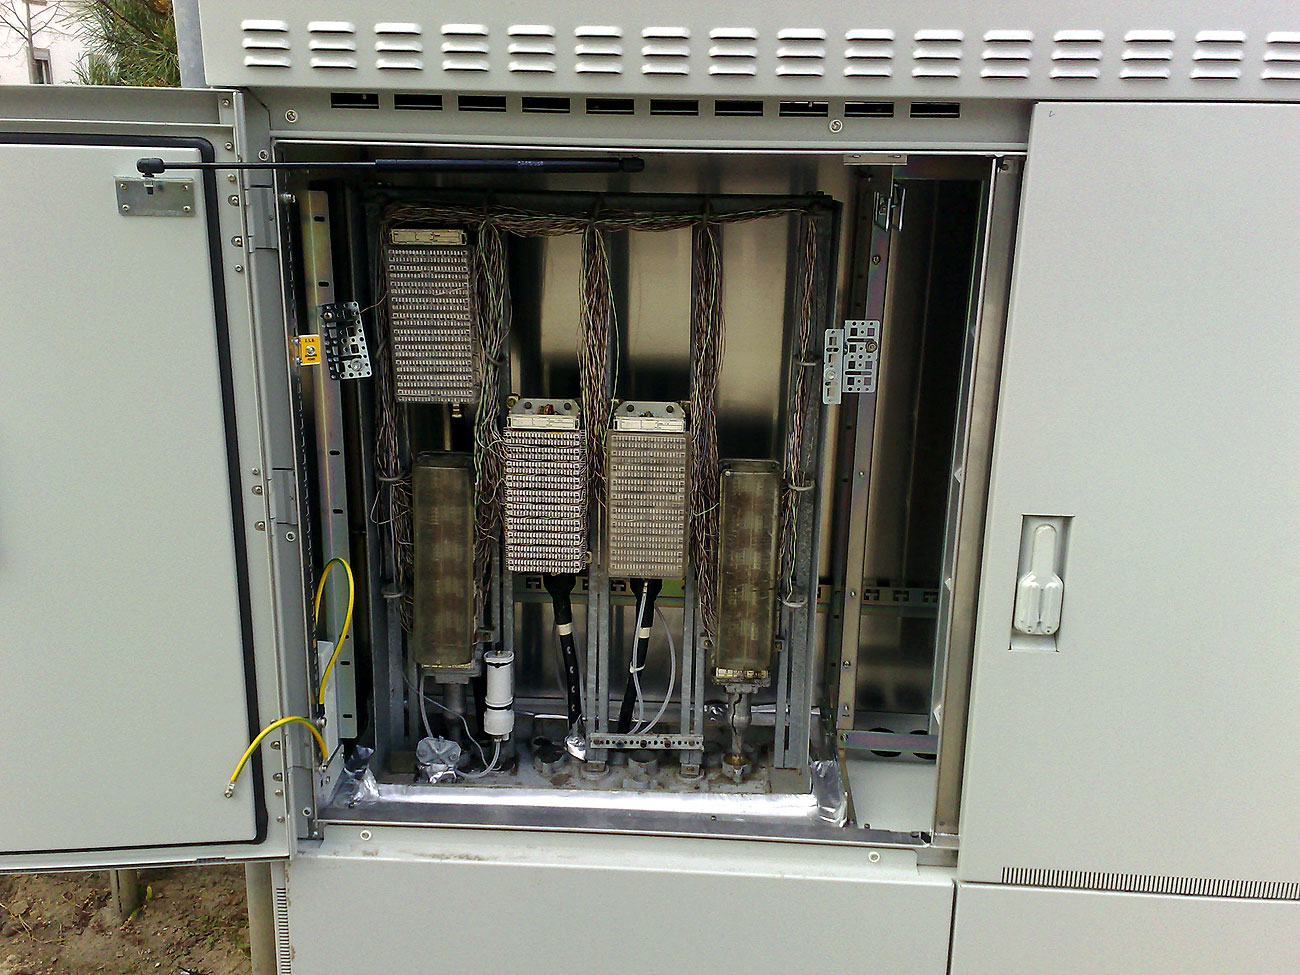
\includegraphics[width=1\textwidth]{assets/chap_2/DSL.png}
\end{minipage}
\end{center}

\noindent
\textbf{Thiết bị:}

\begin{itemize}
    \item Tại gia $\rightarrow$ dùng DSL Modem để giải mã dữ liệu tải về (downstream).
    \item Tại nhà mạng $\rightarrow$ dùng DSLAM (DSL Access Multiplexer - thiết bị ghép kênh truy cập DSL) để gom tín hiệu từ nhà dân lại với nhau.
\end{itemize}

\noindent
\textbf{Đặc điểm kĩ thuật:}

\begin{itemize}
    \item Distance dependency (phụ thuộc vào khoảng cách) $\rightarrow$ tốc độ mạng phụ thuộc vào khoảng cách từ nhà đến trạm DSLAM và chất lượng dân cáp truyền dẫn tín hiệu $\Rightarrow$ nhà càng xa trạm $\rightarrow$ mạng càng chậm và chập chờn.
    \item VDSL2 (Very-high-bit-rate DSL 2) $\rightarrow$ là phiên bản DSL nhanh nhất, có tốc độ lên đến 100 Mbps trong điều kiện khoảng cách ngắn ($<$ 500m) $\rightarrow$ nếu xa hơn sẽ giảm tốc độ đáng kể.
\end{itemize}
\medskip

\subsubsection{Data Over Cable Service Interface Specification (DOCSIS)}

\noindent
DOCSIS (thông số giao diện dịch vụ dữ liệu qua cáp) $\rightarrow$ là chuẩn công nghệ để truyền Internet qua đường dây truyền hình cáp (cable TV).

$\Rightarrow$ Tận dụng hạ tầng $\rightarrow$ sử dụng lại hệ thống cáp đồng trục (coaxial cables) vốn dùng để phát sóng truyền hình cáp.
\medskip

\noindent
\textbf{Thiết bị:}

\begin{center}
\begin{minipage}[c]{0.55\textwidth}
    \begin{itemize}
        \item Tại gia $\rightarrow$ dùng cable modem để nhận tín hiệu (downstream).
        \item Tại nhà mạng $\rightarrow$ dùng hệ thống (CMTS - Cable Modem Termination System) để quản lý tín hiệu gửi lên (upstream).
    \end{itemize}

    \noindent
    $\rightarrow$ Sử dụng các kênh tần số vô tuyến thấp (low-end radio spectrum) (6-8 MHz) để truyền dữ liệu.
\end{minipage}
\hfill
\begin{minipage}[c]{0.35\textwidth}
    \centering
    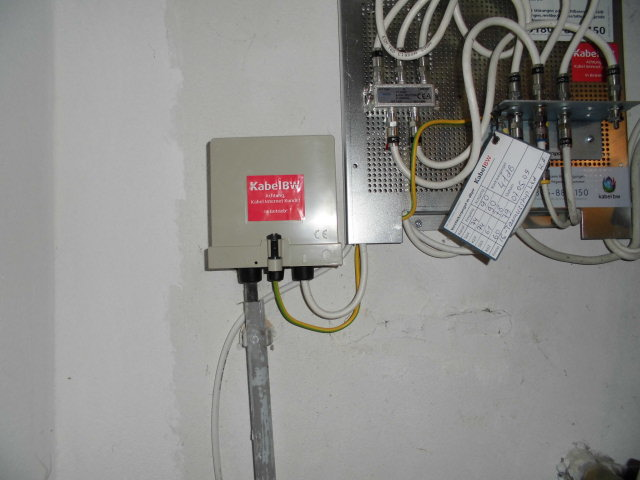
\includegraphics[width=1\textwidth]{assets/chap_2/DOCSIS.png}
\end{minipage}
\end{center}
\medskip

\clearpage

\noindent
\textbf{Đặc điểm kĩ thuật:}

\begin{itemize}
    \item Tốc độ bất đối xứng $\rightarrow$ tải xuống (downstream) lên đến 160 Mbps; trong khi tải lên (upstream) chỉ khoảng 20 Mbps $\Rightarrow$ ưu tiên cho việc lướt web, xem phim (những công việc cần tải về nhiều hơn gửi đi).
    \item Kiến trúc HFC (Hybrid Fiber-Coaxial) $\rightarrow$ các mạng hiện tại dùng kiến trúc lai $\rightarrow$ cáp quang kéo đến khu phố; còn từ khu phố về nhà thì dùng cáp đồng trục $\Rightarrow$ giúp tăng tốc độ.
    \item Shared medium (chia sẻ đường truyền) $\rightarrow$ khác với DSL (đường dây riêng), cáp đồng trục có thể chia sẻ băng thông chung đường truyền.
\end{itemize}

\subsubsection{3GPP Standards}

\noindent
3GPP (3rd Generation Partnership Project) $\rightarrow$ là tổ chức quốc tế chịu trách nhiệm ban hành các chuẩn cho mạng di động (mobile networks) mà mình dùng hằng ngày trên điện thoại.
\medskip

\noindent
Các thế hệ (evolution):

\begin{itemize}
    \item GPRS (2.5G) (General Packet Radio Service) $\rightarrow$ tốc độ rất thấp, tối đa 144 kbps $\rightarrow$ thời kì đầu của Interface di động.
    \item UMTS (3G) (Universal Mobile Telecommunications System) $\rightarrow$ tốc độ nhanh hơn, lên đến 42 Mbps $\rightarrow$ đủ mạnh để có thể lướt web có ảnh, nghe nhạc, bắt đầu gọi video call (nhưng chất lượng thấp, mờ).
    \item LTE (4G) (Long Term Evolution) $\rightarrow$ tốc độ lên đến 168 Mbps $\rightarrow$ dư sức xem HD video, livestream mượt $\Rightarrow$ là chuẩn phổ biến nhất hiện nay.
    \item 5G $\rightarrow$ tốc độ siêu nhanh, lên đến 10 Gbps $\rightarrow$ không chỉ để lướt web, mà còn phục vụ cho mục đích liên quan đến IoT và M2M (machine to machine) $\rightarrow$ phổ biến như xe tự lái, thành phố thông minh.
\end{itemize}
\medskip

\section{Technologies}

\subsection{Standardization}

\noindent
\textbf{Vấn đề:} Tại sao phải cần chuẩn hóa (standardization)?

$\Rightarrow$ Để đảm bảo các thiết bị từ các nhà sản xuất khác nhau có thể hoạt động cùng nhau (interoperability).
\medskip

\noindent
\textbf{$\rightarrow$ Tổ chức quan trọng nhất:} IEEE SA (Institute of Electrical and Electronics Engineers Standards Association) $\rightarrow$ là một cộng đồng trung lập (neutral community), không chịu sự quản lý từ bất kì quốc gia nào.

$\rightarrow$ \textbf{Nhiệm vụ:} ban hành các quy chuẩn kỹ thuật quốc tế.
\medskip

\noindent
\textbf{$\rightarrow$ Bộ tiêu chuẩn trọng điểm:} IEEE 802.
\medskip

\noindent
$\rightarrow$ Là các family of standards dành cho mạng máy tính cục bộ (LAN, PAN, MAN).

\begin{itemize}
    \item \textbf{IEEE 802.1} $\rightarrow$ chuyên về các giao thức mạng lớp cao (higher layer LAN protocols); chẳng hạn như, các vấn đề về cầu nối (bridging), quản lý mạng.
    \item \textbf{IEEE 802.3} $\rightarrow$ là chuẩn cho Ethernet $\Rightarrow$ mọi mạng có dây đều phải tuân theo chuẩn này.
    \item \textbf{IEEE 802.11} $\rightarrow$ là chuẩn mạng cho WLAN (mạng không dây, Wifi) $\Rightarrow$ mọi thiết bị phát Wifi đều phải tuân theo chuẩn này; như 802.11n, 802.11ac, 802.11ax.
    \item \textbf{IEEE 802.15} $\rightarrow$ là chuẩn cho WPAN; chẳng hạn như Bluetooth.
\end{itemize}

\subsection{Ethernet}

\subsubsection{Ethernet (IEEE 802.3)}

\noindent
Ethernet $\rightarrow$ là chuẩn công nghệ cho mạng LAN có dây (wired LAN).

$\rightarrow$ Được phát triển bởi Xerox PARC vào những năm 1970s.
\medskip

\noindent
$\rightarrow$ Với bản vẽ này, Robert Metcalfe đã trình bày nguyên lý hoạt động của Ethernet tại Hội nghị Máy tính Quốc gia vào tháng 6 năm 1976.
\medskip

\begin{figure}[ht]
    \centering
    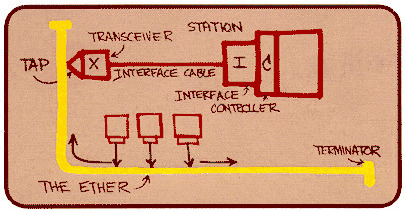
\includegraphics[width=0.55\textwidth]{assets/chap_2/ether.jpg}
\end{figure}
\medskip

\noindent
\textbf{Cách Ethernet hoạt động (xưa):}

\begin{itemize}
    \item The Ether (sợi cáp vàng) $\rightarrow$ là một sợi cáp đồng trục to và dài chạy dọc theo hành lang văn phòng $\Rightarrow$ được gọi là Ether do lấy cảm hứng từ "Ether ánh sáng" (môi trường giả định truyền ánh sáng) $\rightarrow$ ý nói đến dữ liệu lan truyền đi khắp nơi.
    \item Tap (kẹp/mũi khoan) $\rightarrow$ để kết nối máy tính vào mạng thì người ta dùng một thiết bị kẹp chặt và siết thủng vỏ cáp để chạm vào lõi đồng bên trong (hay còn gọi là Vampire tap).
    \item Terminator (nút chặn cuối) $\rightarrow$ hai đầu sợi cáp phải có nút chặn dể tín hiệu không bị dội ngược lại (gây nhiễu đường truyền).
    \item Transceiver and controller (bộ thu phát \& bộ điều khiển) $\rightarrow$ thiết bị thu phát tín hiệu và bo mạch điều khiển.
\end{itemize}

\noindent
$\Rightarrow$ Thông số kỹ thuật của Ethernet $\rightarrow$ bao gồm cả lớp vật lý, và các dịch vụ từ lớp liên kết dữ liệu.
\medskip

\subsubsection{The Evolution of Ethernet}

\noindent
Ethernet đã trải qua nhiều lần nâng cấp theo thời gian:

\begin{itemize}
    \item 1973 $\rightarrow$ Ethernet chính thức được phát triển tại Xerox PARC bởi Robert Metcalfe và các cộng sự $\rightarrow$ tốc độ 2.94 Mbps, sử dụng cáp đồng trục.
    \item 1983 $\rightarrow$ IEEE ban hành thông số kĩ thuật cho 10BASE5 (còn được gọi là thick Ethernet) $\rightarrow$ dùng cáp đồng trục to, tốc độ khoảng 10 Mbps $\Rightarrow$ khó lắp đặt do cáp cứng, phải khoang lỗ (như hình trên mô tả).
    \item 1988 $\rightarrow$ AT\&T ra mắt StarLAN 10 (the basis của 10BASE-T) $\rightarrow$ chuyển sang dùng cáp xoắn đôi (twisted pair) mềm dẻo, dễ lắp đặt hơn.
    \item 1990 $\rightarrow$ Ethernet trở thành công nghệ mạng LAN có dây (wired LAN) được sử dụng phổ biến trên thế giới.
    \item Mạng ngày nay có thể đạt đến 1 Tbps, sử dụng đa dạng phương thức truyền khác nhau như cáp đồng trục, cáp xoắn đôi, cáp quang.
\end{itemize}
\medskip

\subsection{Wireless Local Area Network (WLAN)}

\subsubsection{WLAN (IEEE 802.11)}

\noindent
\textbf{Tổng quan:}

\begin{itemize}
    \item Tên chuẩn $\rightarrow$ IEEE 802.11.
    \item Tên thương mại $\rightarrow$ Wifi (Wireless Fidelity) $\Rightarrow$ đây là tên thường gọi chứ không phải là tên kĩ thuật.
    \item Là công nghệ mạng không dây phổ biến nhất hiện nay.
    \item Các chuẩn hiện tại có thể đạt tốc độ lên đến 7 Gbps.
\end{itemize}
\medskip

\noindent
\textbf{Các mô hình kết nối (communication models):}

\begin{itemize}
    \item \textbf{Infrastructure mode} (chế độ hạ tầng) $\rightarrow$ tất cả các thiết bị (clients) kết nối vào một cục phát sóng trung tâm gọi là access point (AP) $\Rightarrow$ đây là cách dùng phổ biến nhất, muốn vào mạng thì phải có cục Router/AP.
    \item \textbf{Ad-hoc mode} (chế độ tự phát) $\rightarrow$ các thiết bị kết nối trực tiếp với nhau tạo thành một mạng lưới (mesh network), không cần cục AP trung tâm; chẳng hạn như chuyển file qua AirDrop.
\end{itemize}

\subsubsection{The Evolution of WLAN standards}

\begin{itemize}
    \item 1995 $\rightarrow$ US FFC (Federal Communications Commission) giải phóng băng tần ISM (Industrial, Scientific, and Medical) cho công chúng miễn phí, bao gồm dải tần 2.4 GHz.
    \item 1997 $\rightarrow$ chuẩn 802.11 đầu tiên ban hành.
    \item 1999 $\rightarrow$ chuẩn 802.11b ban hành với tốc độ lên đến 11 Mbps.
    \item[$\rightarrow$] Sau đó, các chuẩn như 802.11a hoặc 802.11n được ban hành, mở rộng dải tần 5 GHz $\Rightarrow$ tránh bị tắc nghẽn.
\end{itemize}

\begin{table}[H]
    \renewcommand{\arraystretch}{1.2}
    \begin{tabular*}{\linewidth}{@{\extracolsep{\fill}}lcc}
        \hline
        \textbf{IEEE Standard} & \textbf{Maximum (gross) Data Rate} & \textbf{Realistic (net) Data Rate} \\
        \hline
        802.11   & 2 Mbps       & 1 Mbps        \\
        802.11a  & 54 Mbps      & 20--22 Mbps   \\
        802.11b  & 11 Mbps      & 5--6 Mbps     \\
        802.11g  & 54 Mbps      & 20--22 Mbps   \\
        802.11n  & 600 Mbps     & 200--250 Mbps \\
        802.11ac & 1.733 Gbps   & 800--850 Mbps \\
        \hline
    \end{tabular*}
\end{table}
\medskip

\sidebox[-8cm]{Self-note:}{
\begin{itemize}
    \item Gross data rate (tốc độ tổng) $\rightarrow$ tốc độ truyền dữ liệu theo lý thuyết, không có nhiễu hay các tác nhân ngoại vi ảnh hưởng.
    \item Net data rate (tốc độ thực) $\rightarrow$ tốc độ thực tế đo được khi có ngoại vi gây ảnh hưởng đến đường truyền.
\end{itemize}
\medskip

\noindent
$\Rightarrow$ Do nhiễu, gửi kèm các header, sửa lỗi, ... nên sẽ bị giảm tốc độ so với lý thuyết $\rightarrow$ hiệu suất thực tế chỉ đạt khoảng 30-50\% so với lý thuyết.
}

\subsubsection{Non-overlapping Channels of IEEE 802.11b}

\noindent
Các kênh không chồng lấn (non-overlapping channels) $\rightarrow$ là vấn đề nan giải nhất của Wifi băng tần 2.4 GHz.
\medskip

\begin{figure}[H]
    \centering
    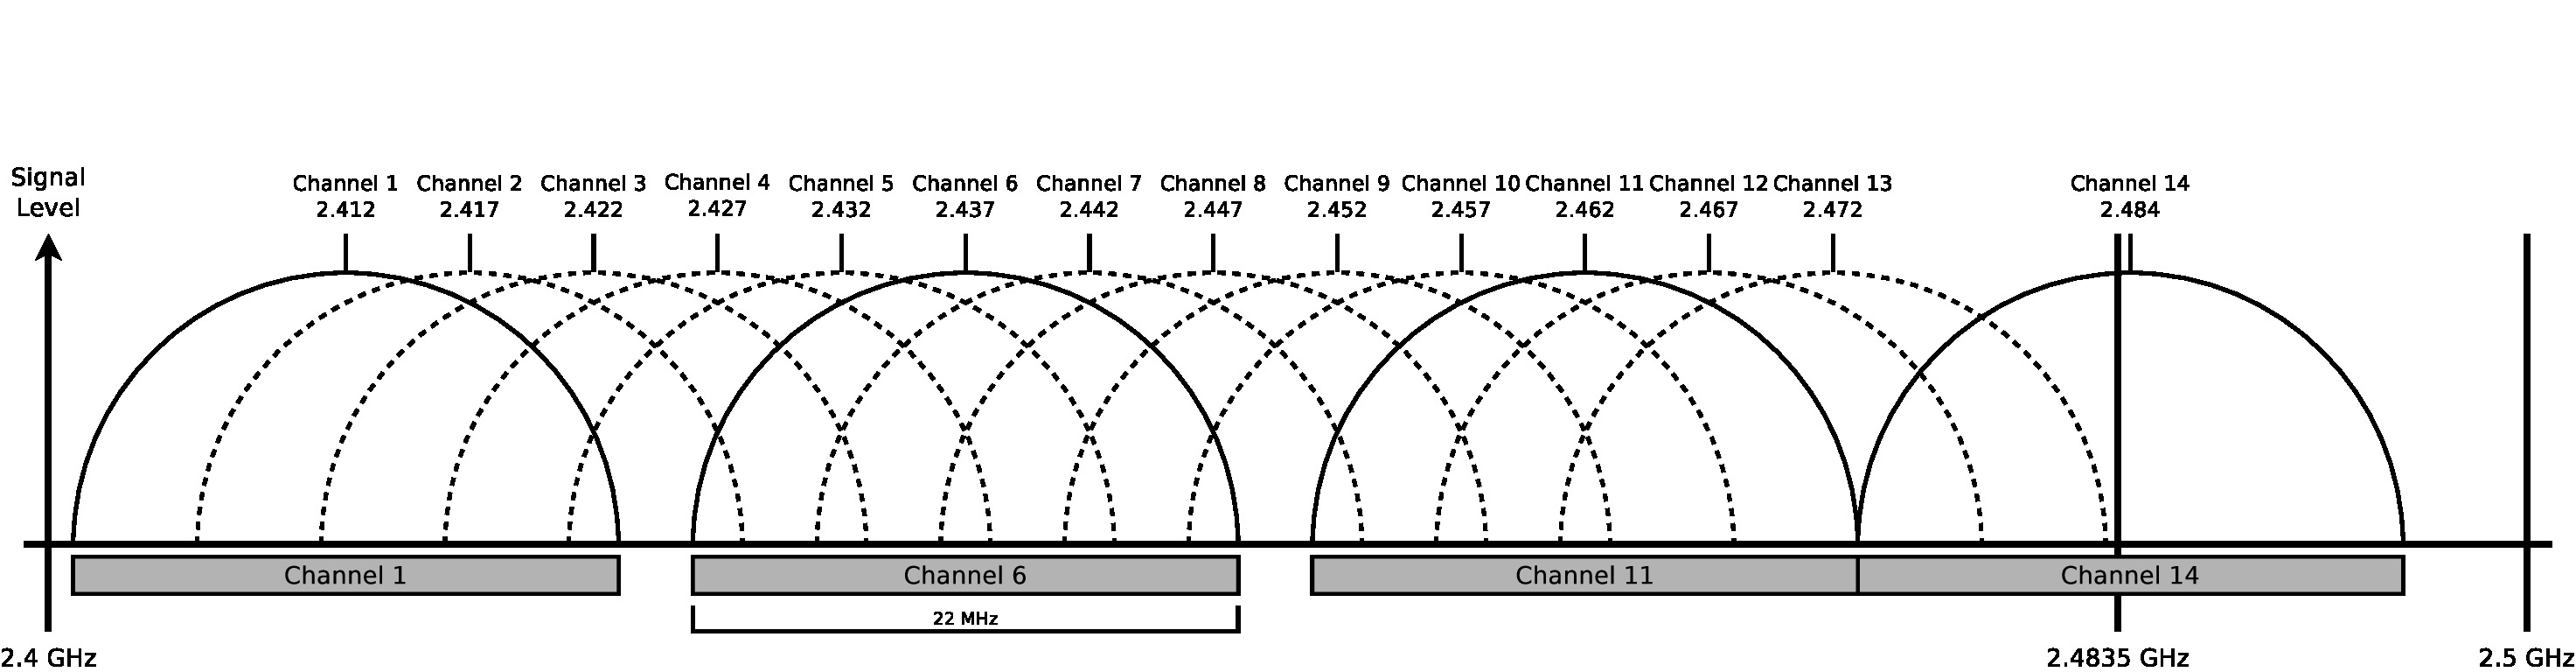
\includegraphics[width=0.8\textwidth]{assets/chap_2/non-overlap.jpg}
\end{figure}
\medskip

\begin{itemize}
    \item Tần số (nằm ở trục ngang) $\rightarrow$ dải tần 2.4 GHz được chia thành 11 đến 14 kênh nhỏ, mỗi kênh cách nhau 5 MHz.
    \item Độ rộng kênh $\rightarrow$ mỗi kênh Wifi cần một khoảng rộng 22 MHz để hoạt động.
    \item[$\Rightarrow$] Do các kênh được đặt quá sát nhau (cách nhau 5 MHz), trong khi cái độ rộng quá to (22 MHz) $\rightarrow$ kênh 1 sẽ lấn sang chỗ của kênh 2, 3, 4, 5.
\end{itemize}
\medskip

\noindent
Dải tần 2.4 GHz được chia thành các kênh (channels), mỗi kênh rộng 22 MHz nhưng chỉ cách nhau 5 MHz $\rightarrow$ các kênh nằm cạnh sẽ đè lên nhau (overlapping).
\medskip

\noindent
\textbf{$\rightarrow$ Giải pháp:} chỉ có 3 kênh duy nhất là không bị chồng lên nhau là 1, 6, và 11 $\Rightarrow$ trong một khu vực dày đặc người dùng, nếu người đầu tiên dùng kênh 1, còn người thứ hai dùng kên 2 $\rightarrow$ bị nhiễu $\Rightarrow$ người thứ hai phải bắt buộc đổi sang kênh 6 hoặc 11 để dùng được mạng tốt hơn.

$\Rightarrow$ Quy tắc 1-6-11 $\rightarrow$ để không bị chồng lên nhau, mình phải chọn các kênh cách xa nhau $\rightarrow$ chỉ có bộ ba 1-6-11 là hoàn toàn cách xa nhau, không chồng lấn lên nhau (như hình trên mô tả).
\medskip

\sidebox[-2cm]{Fact:}{Ở Nhật nó có có kênh 14, nghĩa là nó có tới tận 4 kênh không chồng lấn (1, 6, 11, 14).}

\subsubsection{WLAN Security: WEP and WPA}

\noindent
\textbf{WEP (Wired Equivalent Privacy)} $\rightarrow$ là chuẩn bảo mật đời đầu của Wifi.

$\Rightarrow$ Sử dụng khóa tĩnh (static keys) với độ dài 40-bit hoặc 104-bit $\rightarrow$ đã suspended do rất dễ bị hack; phần đầu gói tin (protocol header) có quy luật dễ đoán nên có thể bẻ khóa trong thời gian cực ngắn.
\medskip

\noindent
\textbf{WPA (Wi-Fi Protected Access)} $\rightarrow$ là chuẩn bảo mật thay thế WEP; có các phiên bản WPA 1, 2, và 3.

\begin{itemize}
    \item WPA1 $\rightarrow$ dùng thuật toán mã hóa RC4 (Rivest Cipher 4) $\Rightarrow$ hiện tại không còn an toàn nữa.
    \item WPA2 (phổ biến ngày nay) $\rightarrow$ dùng thuật toán AES (Advanced Encryption Standard) $\Rightarrow$ rất an toàn nếu đặt mật khẩu đủ dài và khó đoán.
\end{itemize}

\noindent
\textbf{Các phương thức xác thực (key distribution)} $\rightarrow$ làm sao để đưa key cho người dùng?

\begin{itemize}
    \item PSK (Pre-Shared Key) $\rightarrow$ dùng chung một mật khẩu cho tất cả mọi người $\rightarrow$ dùng ở nhà (WPA-Personal).
    \item WPA-Enterprise $\rightarrow$ sử dụng một máy chủ xác thực riêng (RADIUS server - Remote Authentication Dial-In User Service) $\rightarrow$ mỗi người dùng sẽ có một tài khoản và mật khẩu riêng để đăng nhập (như Eduroam trong FRA-UAS).
    \item WPS (Wifi-Protected Setup) $\rightarrow$ kết nối nhanh bằng cách bấm nút trên Router hoặc nhập mã PIN, không cần gõ mật khẩu dài dòng.
\end{itemize}

\noindent
\textbf{Tổng quan về thuật toán RC4 và AES:}

\begin{itemize}
    \item RC4 $\rightarrow$ tạo ra một dòng các bit ngẫu nhiên vô tận (keystream), sau đó lấy dòng này XOR với các bit dữ liệu để mã hóa $\Rightarrow$ do sử dụng XOR nên nó tính reverse, nghĩa là nếu mà lấy được 2 gói tin được mã hóa bằng cùng một đoạn keystream (do nó lặp lại) $\rightarrow$ có thể dùng XOR để loại bỏ khóa và tìm ra dữ liệu gốc dễ dàng.
    \item AES $\rightarrow$ nó không mã hóa từng bit, mà cắt dữ liệu thành các khối vuông (ví dụ như 4x4 ô), sau đó thực hiện các phép biến đổi phức tạp: ShiftRows, SubBytes, MixColumns, lặp đi lặp lại nhiều lần. $\Rightarrow$ phá vỡ hoàn toàn cấu trúc của dữ liệu gốc $\rightarrow$ một thay đổi nhỏ ở đầu vào sẽ làm thay đổi toàn bộ khối dữ liệu đầu ra (Avalanche Effect - hiệu ứng tuyết lở).
\end{itemize}

\begin{mybox}{Công thức RC4}
$\text{Ciphertext} = \text{Plaintext} \oplus \text{Keystream}$
\end{mybox}
